
\begin{frame}
    \frametitle{Problem definition}
    Aim is to estimate the distribution of English alphabets in a set of
    books and check if it is approaching Normal distribution in Probability. \\

    \vspace{0.5cm}

    The following books were taken for this work
    \begin{itemize}
        \item Animal Farm, by George Orwell
        \item Around the world in eighty days, by Jules Verne
        \item Flow, by Philip Ball
        \item For the love of Physics, by Walter Lewin
        \item Ikigai, by Hector Garcia and Francesc Miralles
        \item The power of positive thinking, by Norman Vincent
    \end{itemize}
\end{frame}

\begin{frame}
    \frametitle{Solution approach}
    A couple of Python codes were generated to read pdf files and process line-wise
    data with the following Pseudocode.
    \begin{figure}
        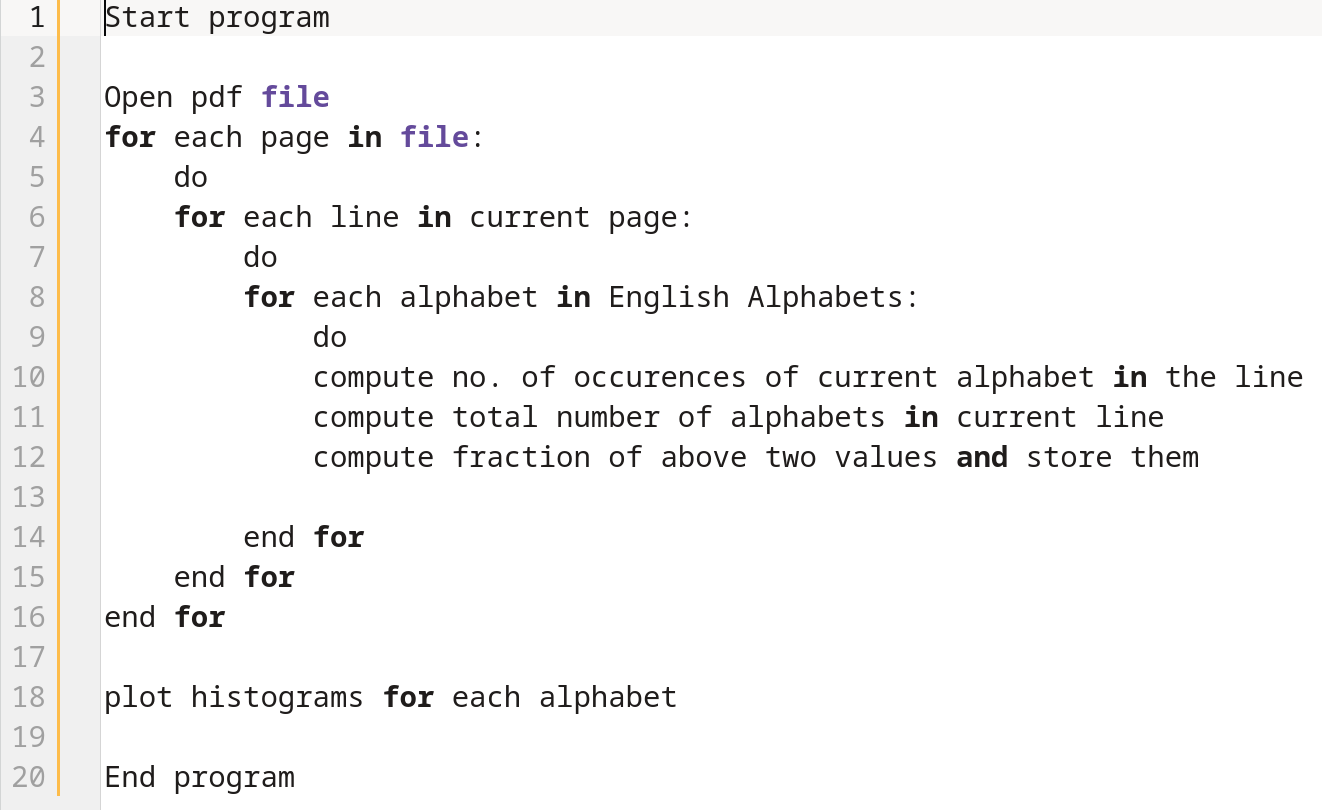
\includegraphics[scale=0.22]{pseudocode.png}
    \end{figure}
\end{frame}

%------------------------------------------------------------------------------
\begin{frame}
    \centering
    \usebeamercolor[fg]{title}\usebeamerfont{title} Histograms of all alphabets \\ compared against \\ all chosen books
\end{frame}

\begin{frame}
    \frametitle{A or a}
    \begin{center}
        \hspace*{-5ex}
        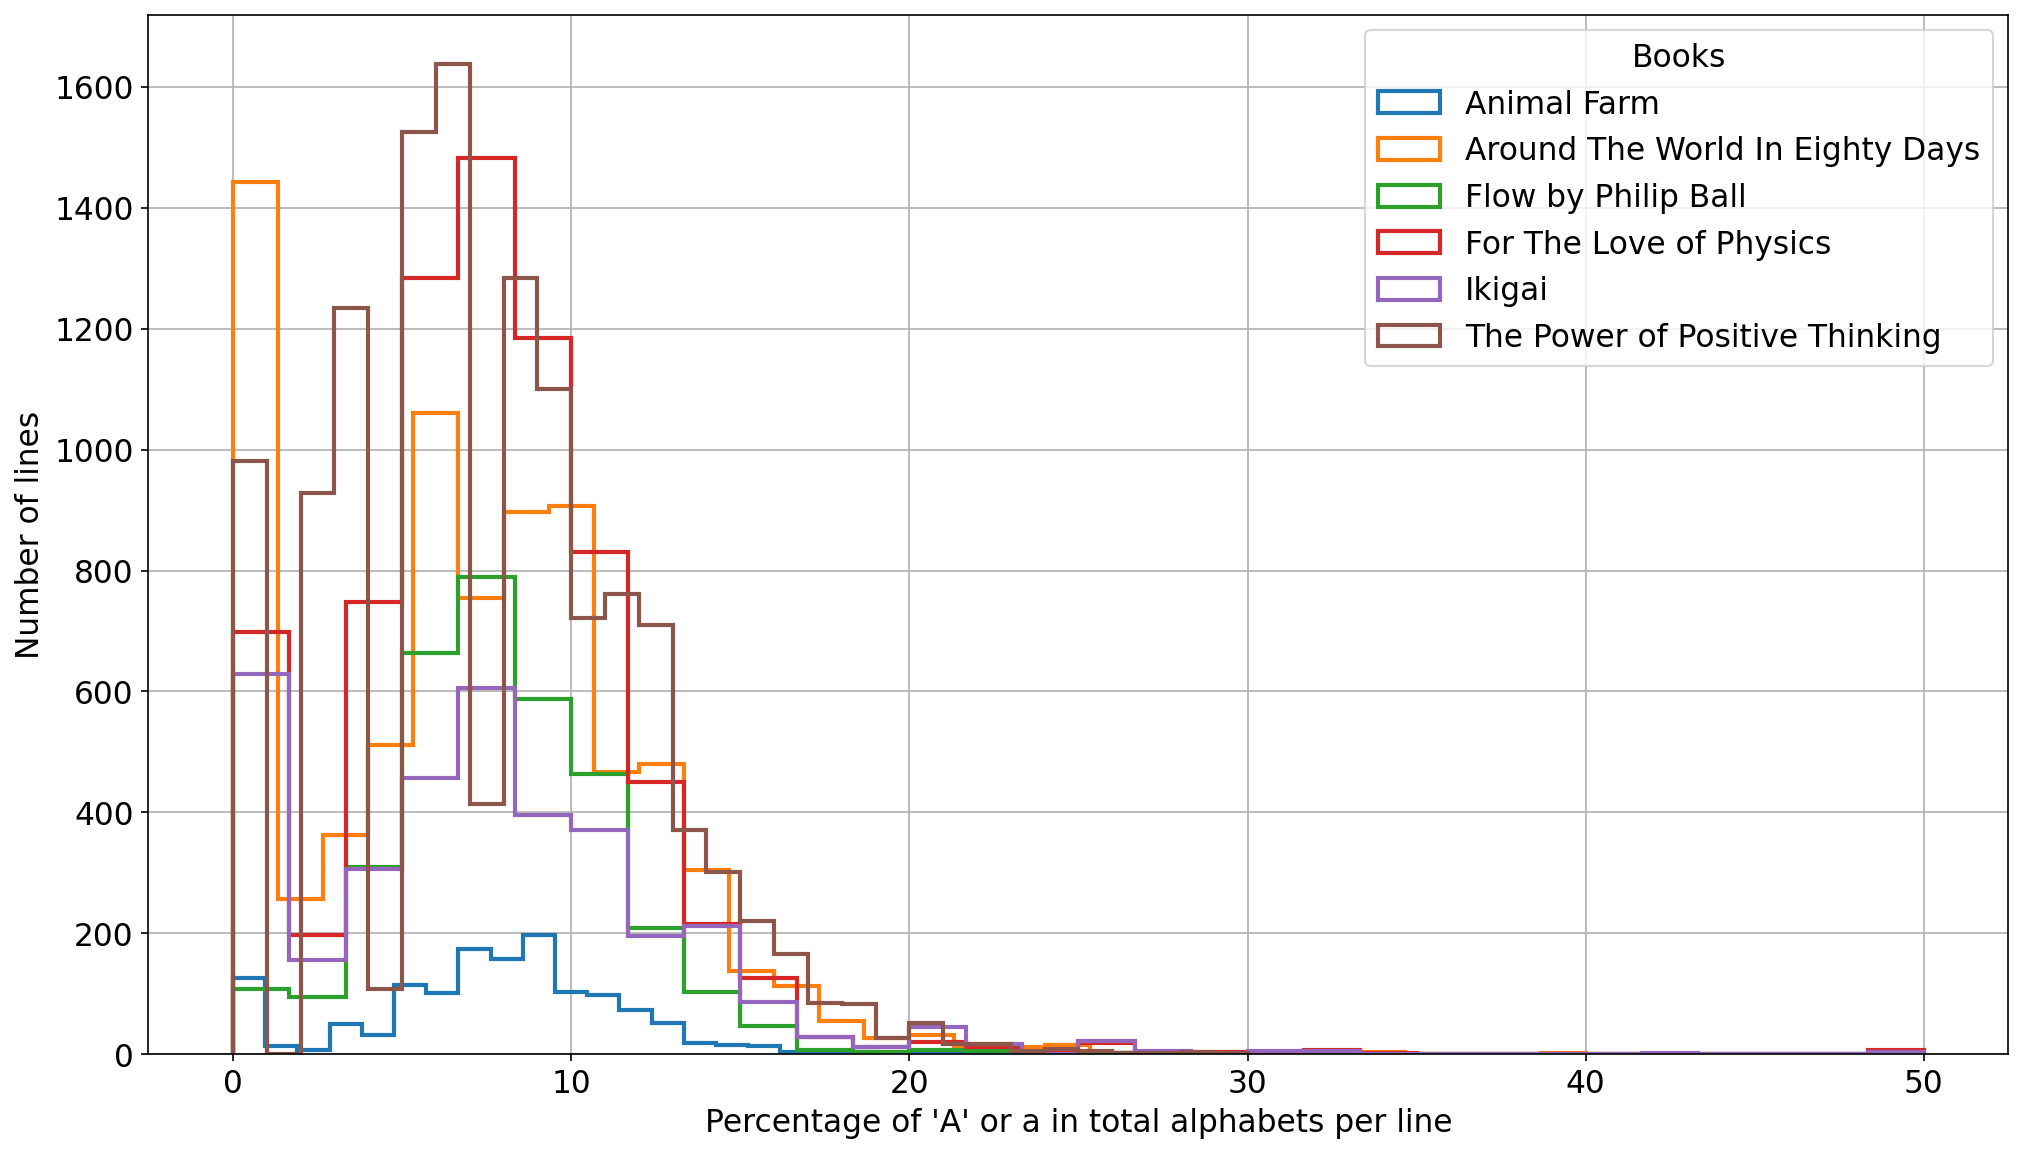
\includegraphics[scale=0.35]{../01_programFiles/histograms/a.png}\hspace{10ex}
    \end{center}
\end{frame}

\begin{frame}
    \frametitle{B or b}
    \begin{center}
        \hspace*{-5ex}
        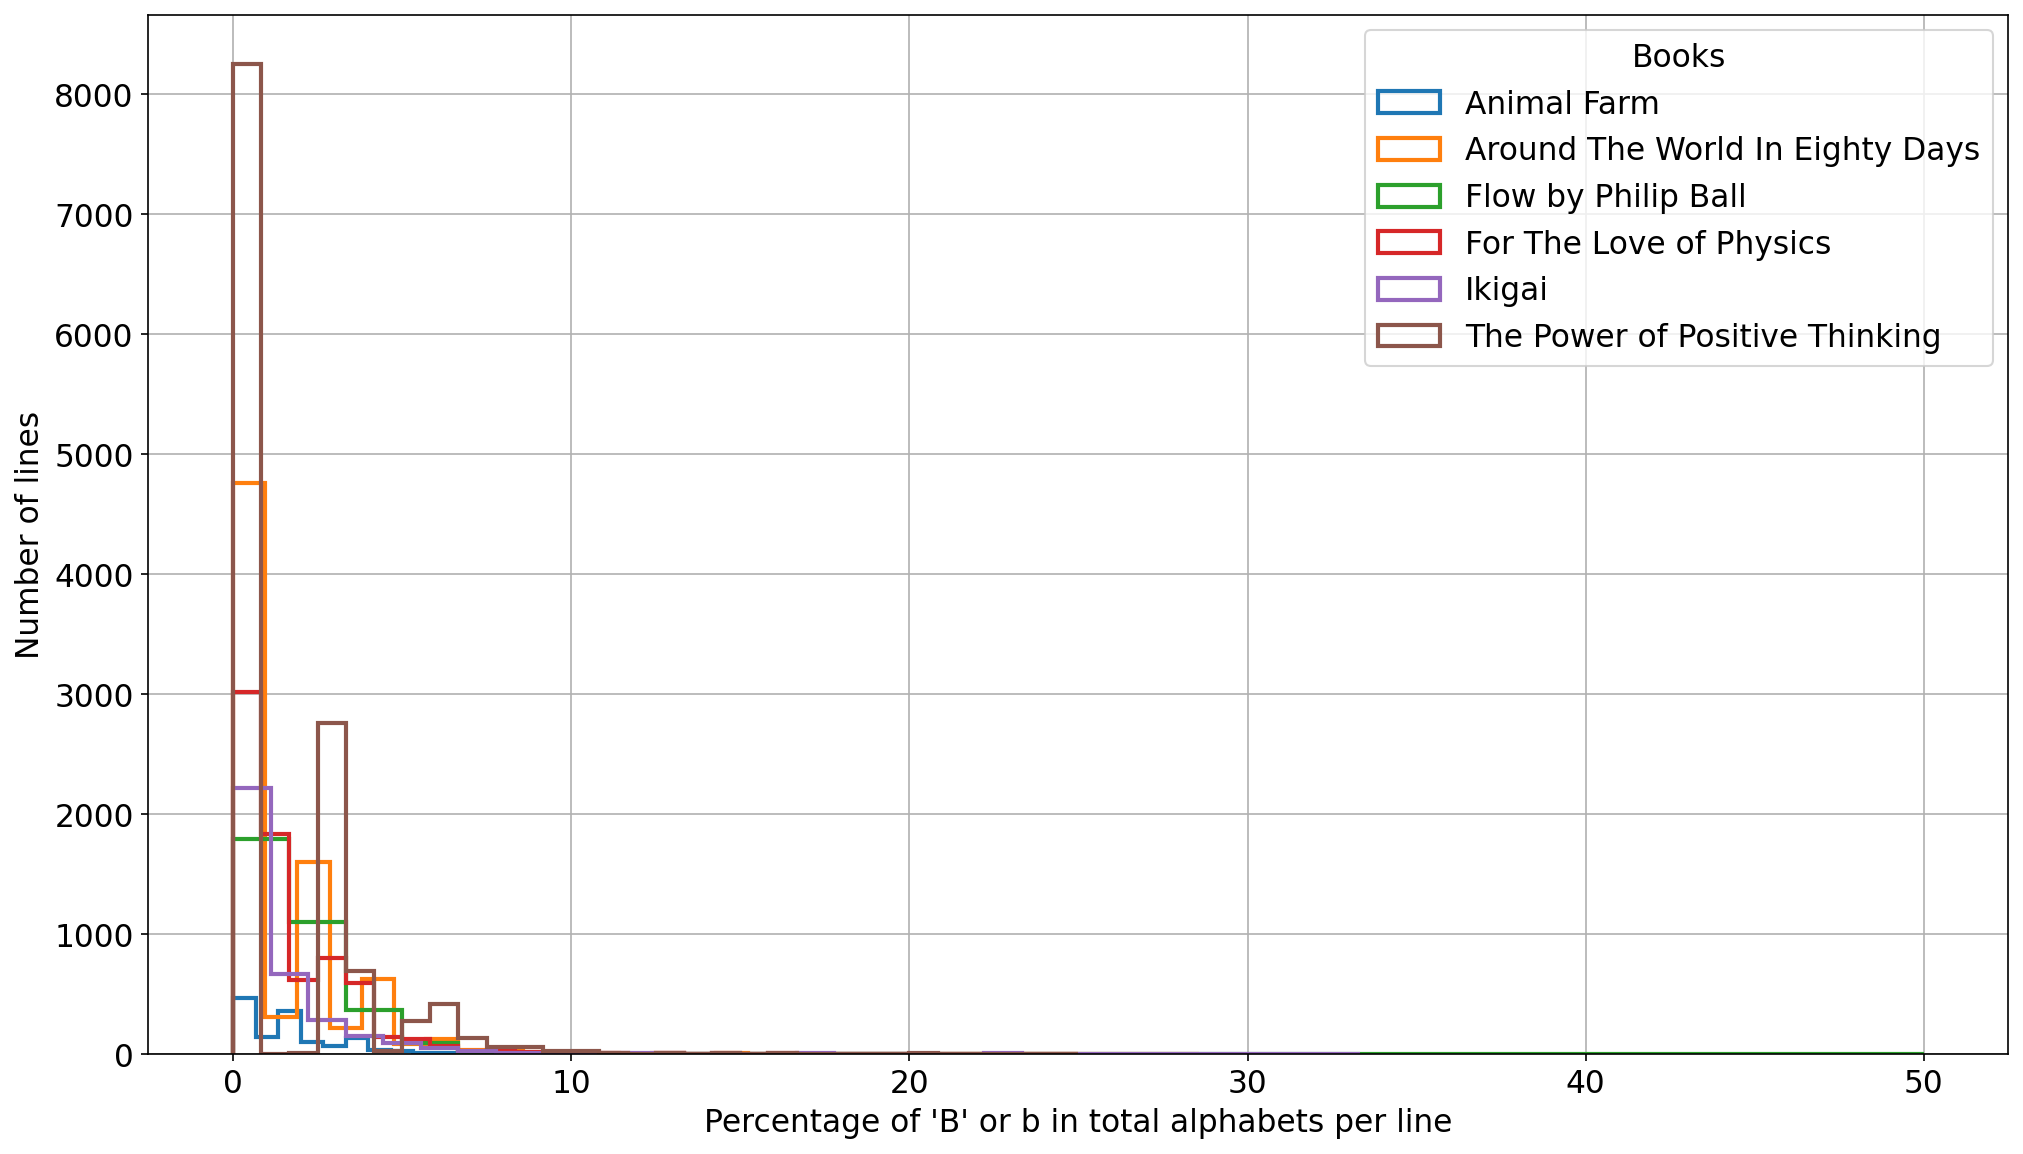
\includegraphics[scale=0.35]{../01_programFiles/histograms/b.png}\hspace{10ex}
    \end{center}
\end{frame}

\begin{frame}
    \frametitle{C or c}
    \begin{center}
        \hspace*{-5ex}
        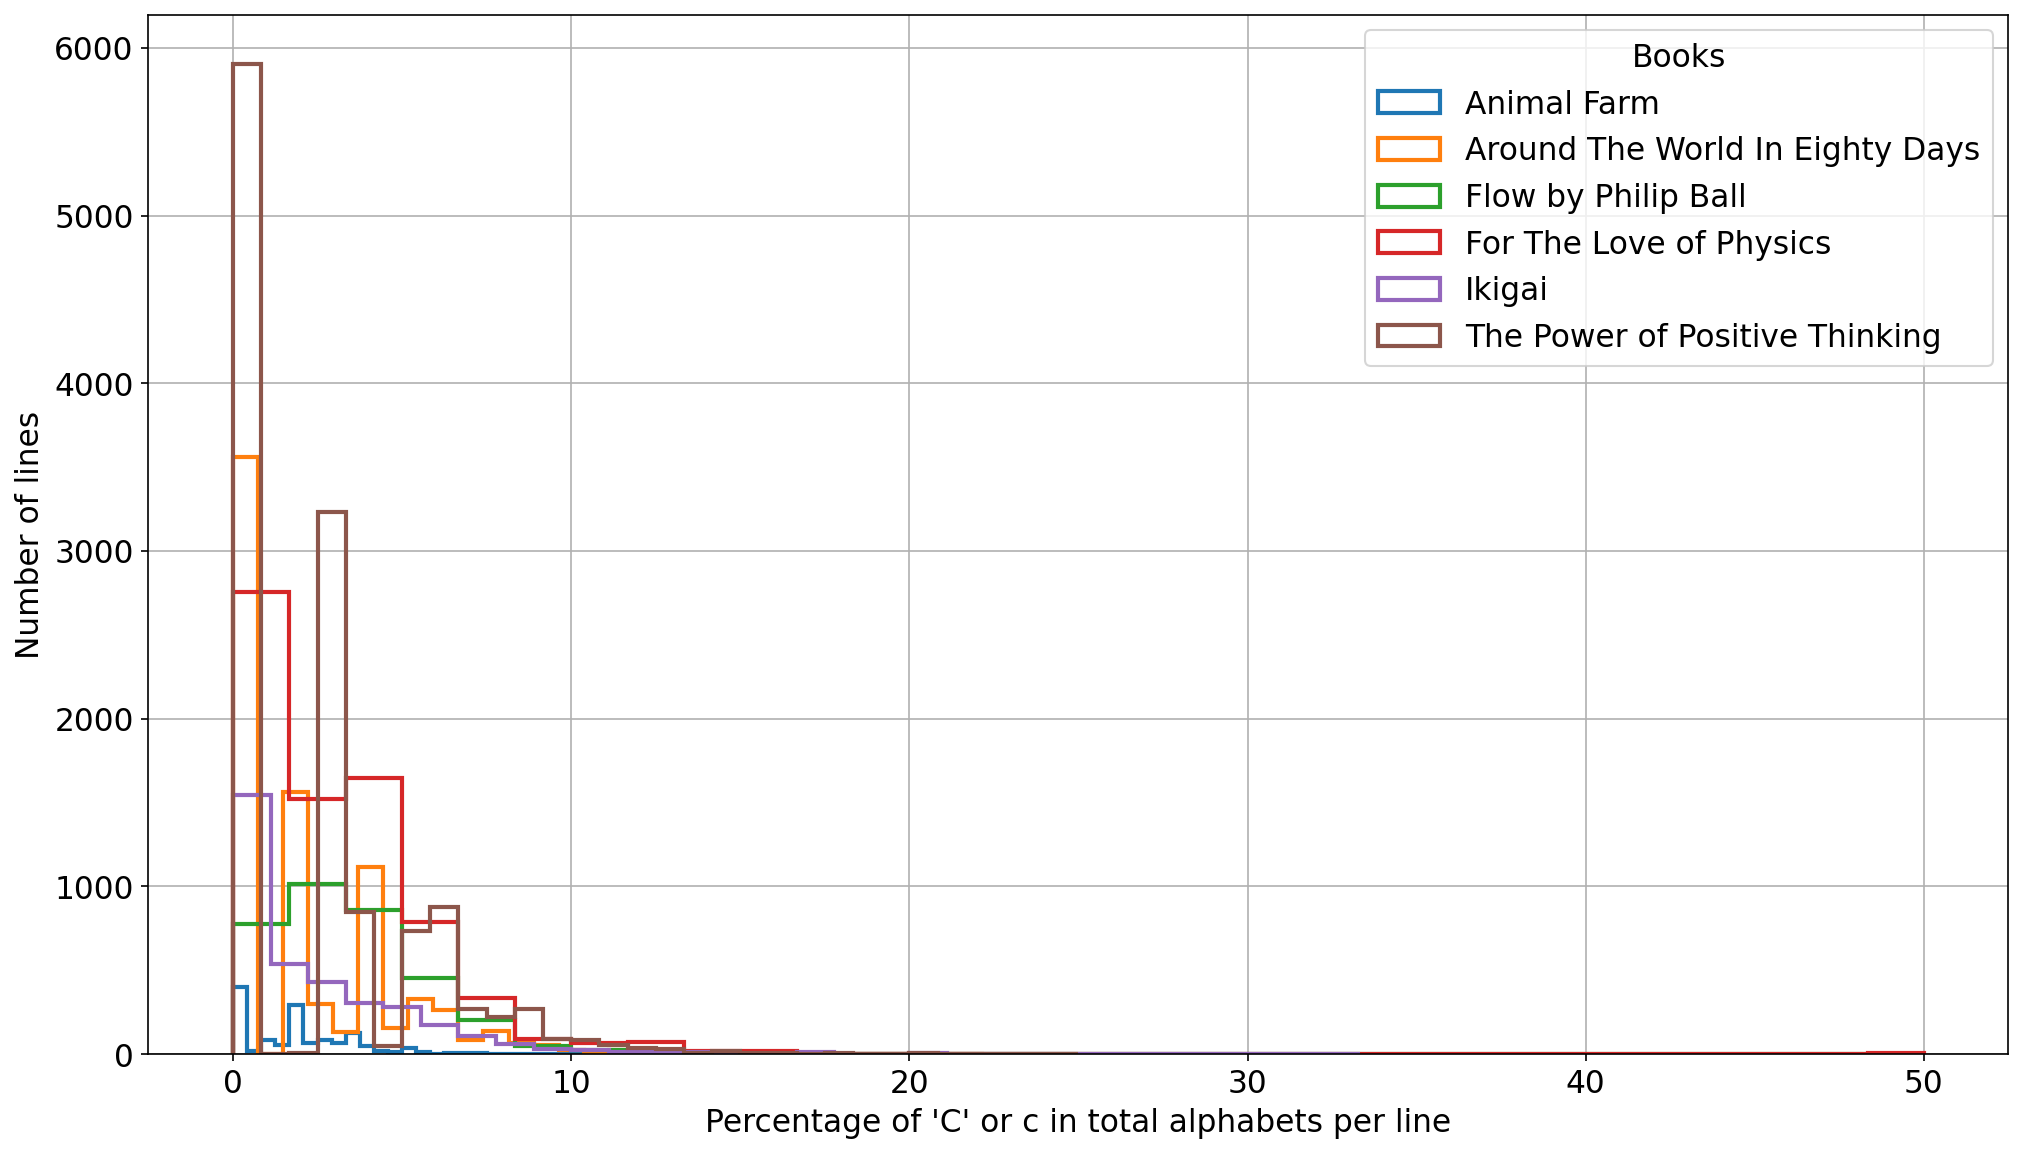
\includegraphics[scale=0.35]{../01_programFiles/histograms/c.png}\hspace{10ex}
    \end{center}
\end{frame}

\begin{frame}
    \frametitle{D or d}
    \begin{center}
        \hspace*{-5ex}
        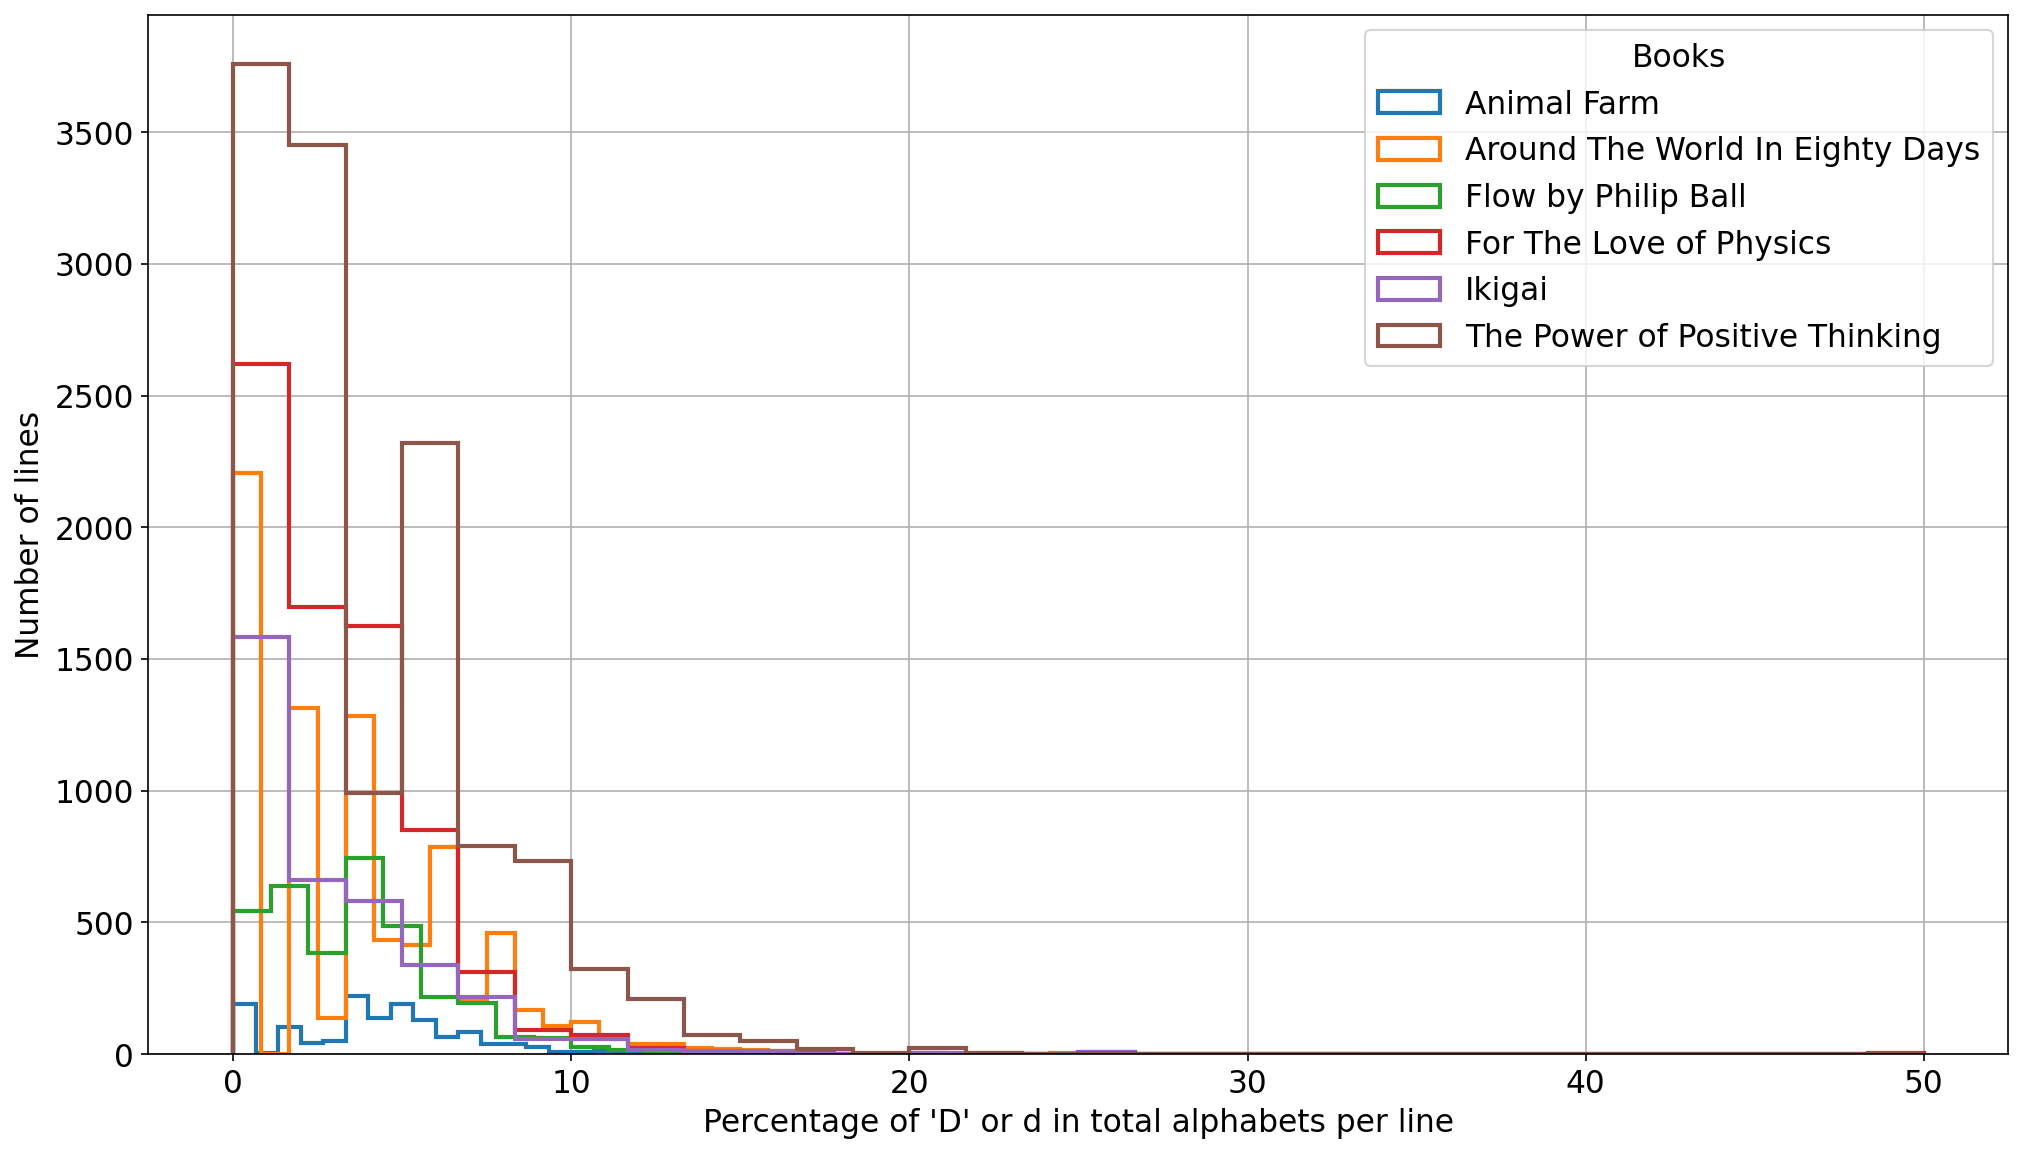
\includegraphics[scale=0.35]{../01_programFiles/histograms/d.png}\hspace{10ex}
    \end{center}
\end{frame}

\begin{frame}
    \frametitle{E or e}
    \begin{center}
        \hspace*{-5ex}
        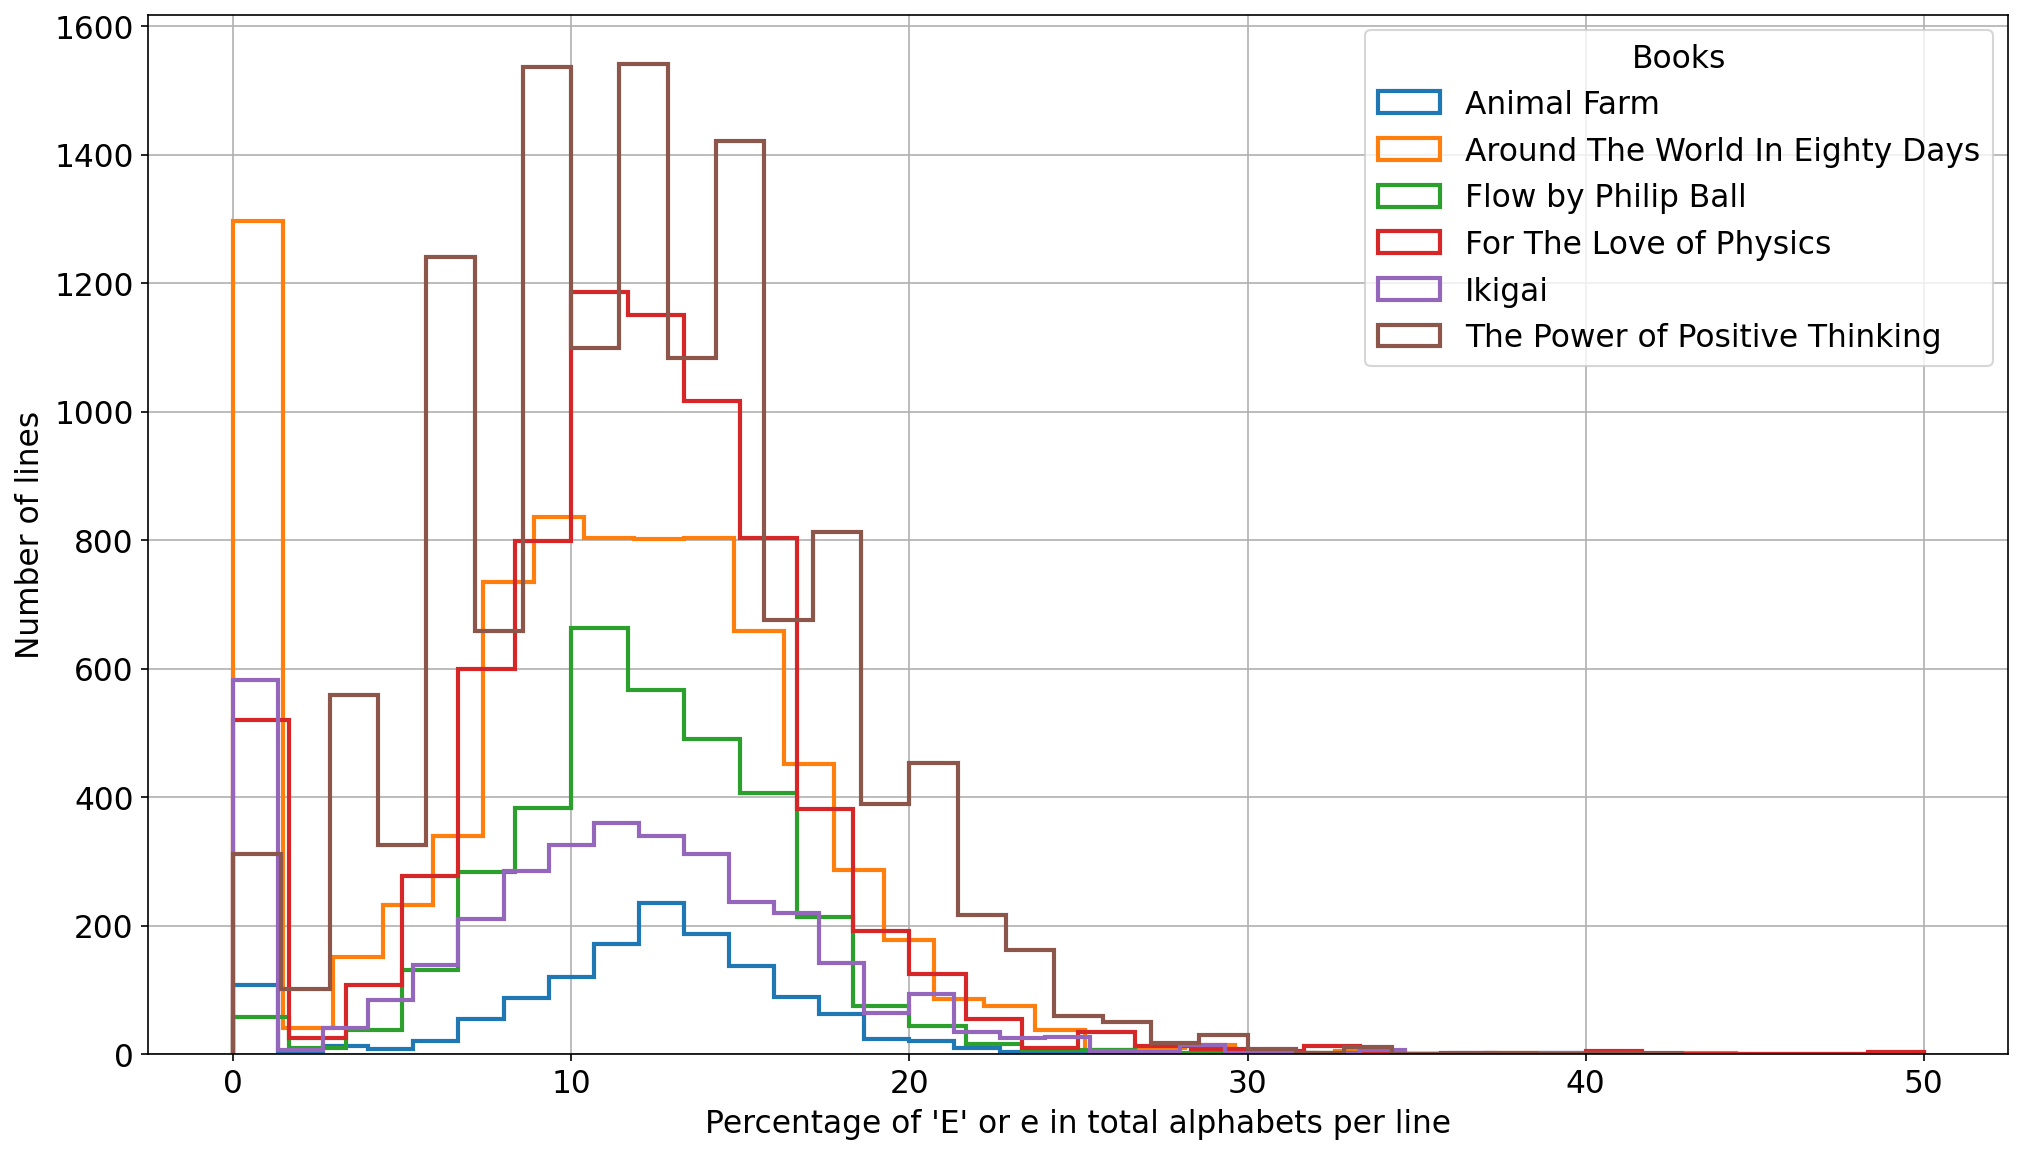
\includegraphics[scale=0.35]{../01_programFiles/histograms/e.png}\hspace{10ex}
    \end{center}
\end{frame}

\begin{frame}
    \frametitle{F or f}
    \begin{center}
        \hspace*{-5ex}
        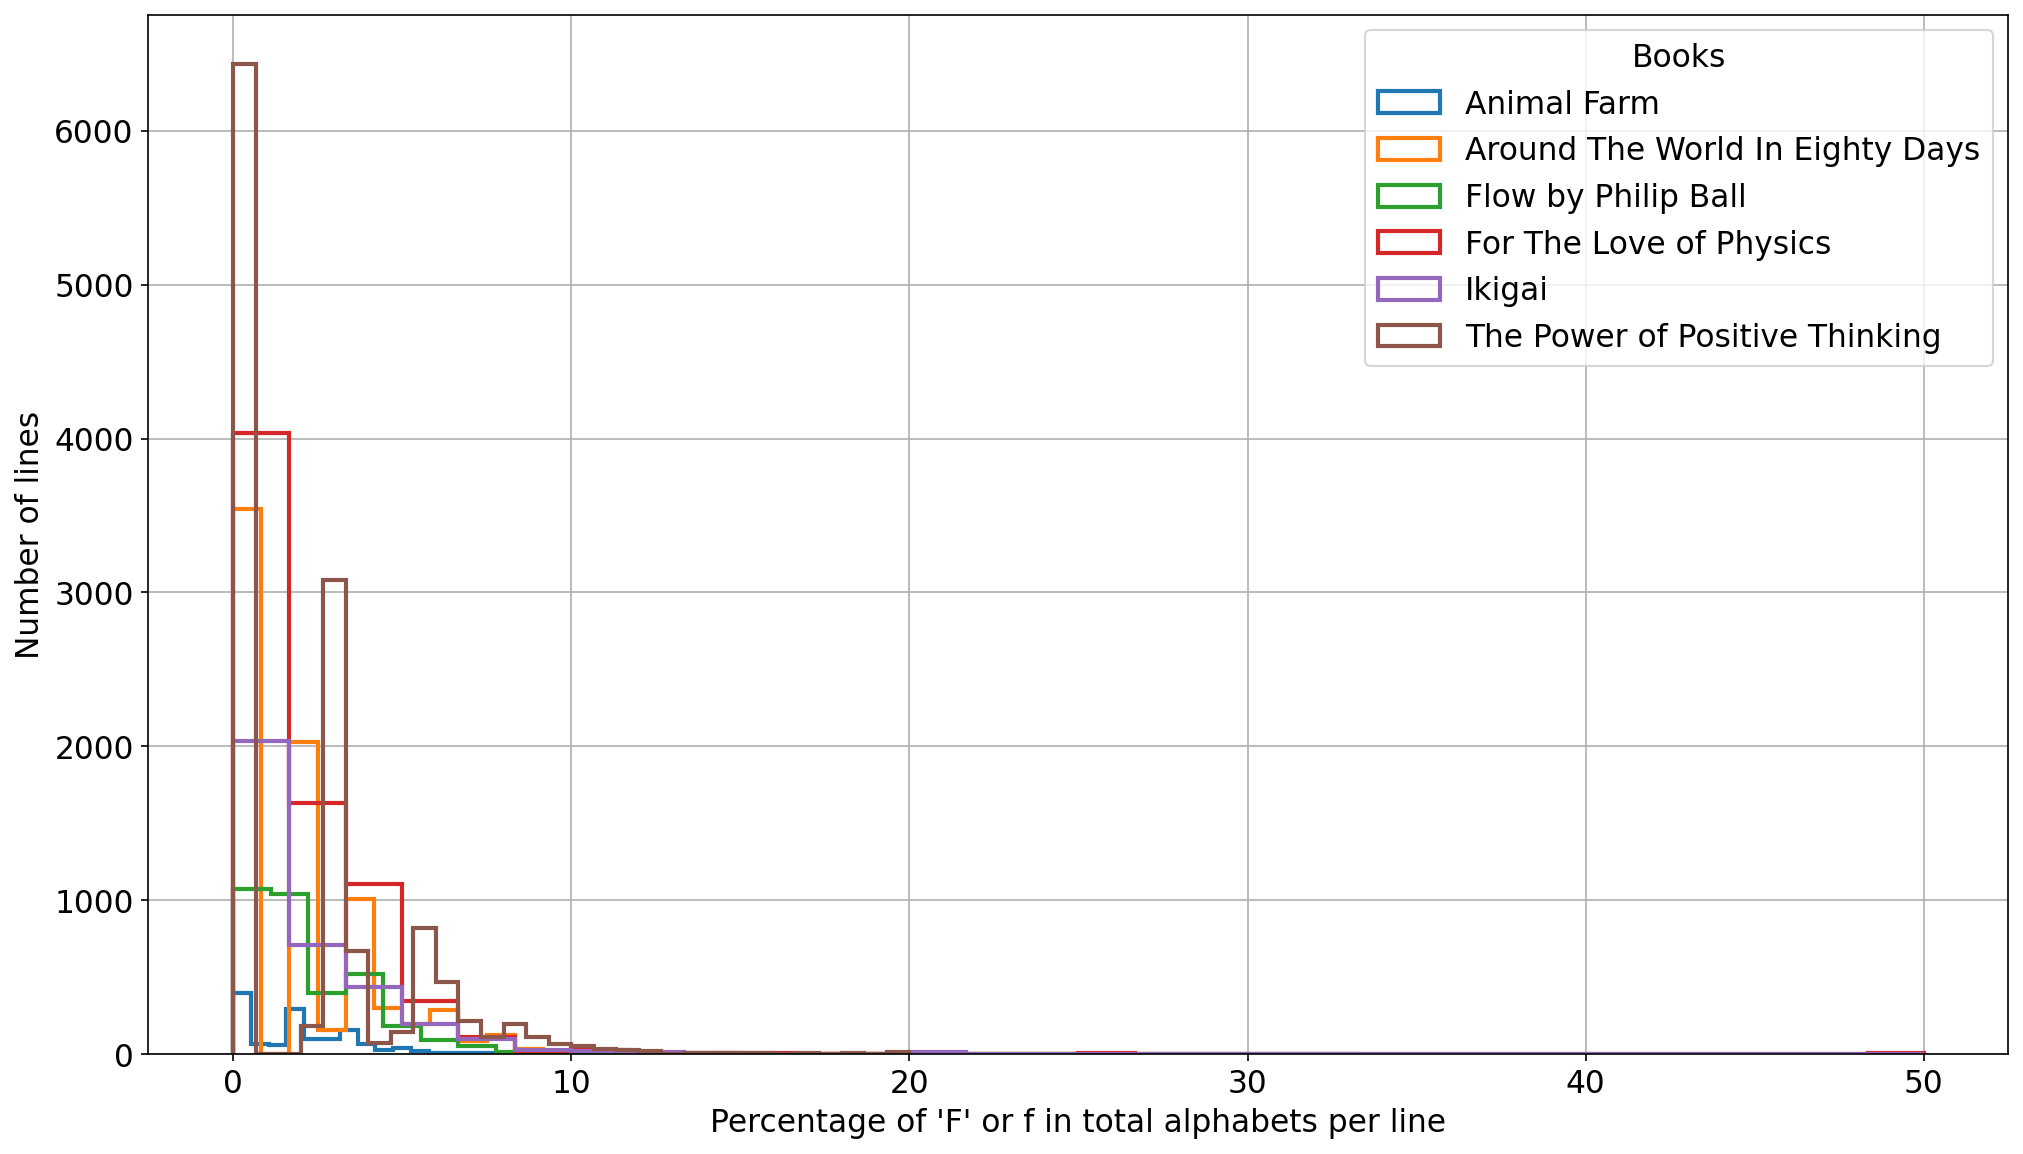
\includegraphics[scale=0.35]{../01_programFiles/histograms/f.png}\hspace{10ex}
    \end{center}
\end{frame}

\begin{frame}
    \frametitle{G or g}
    \begin{center}
        \hspace*{-5ex}
        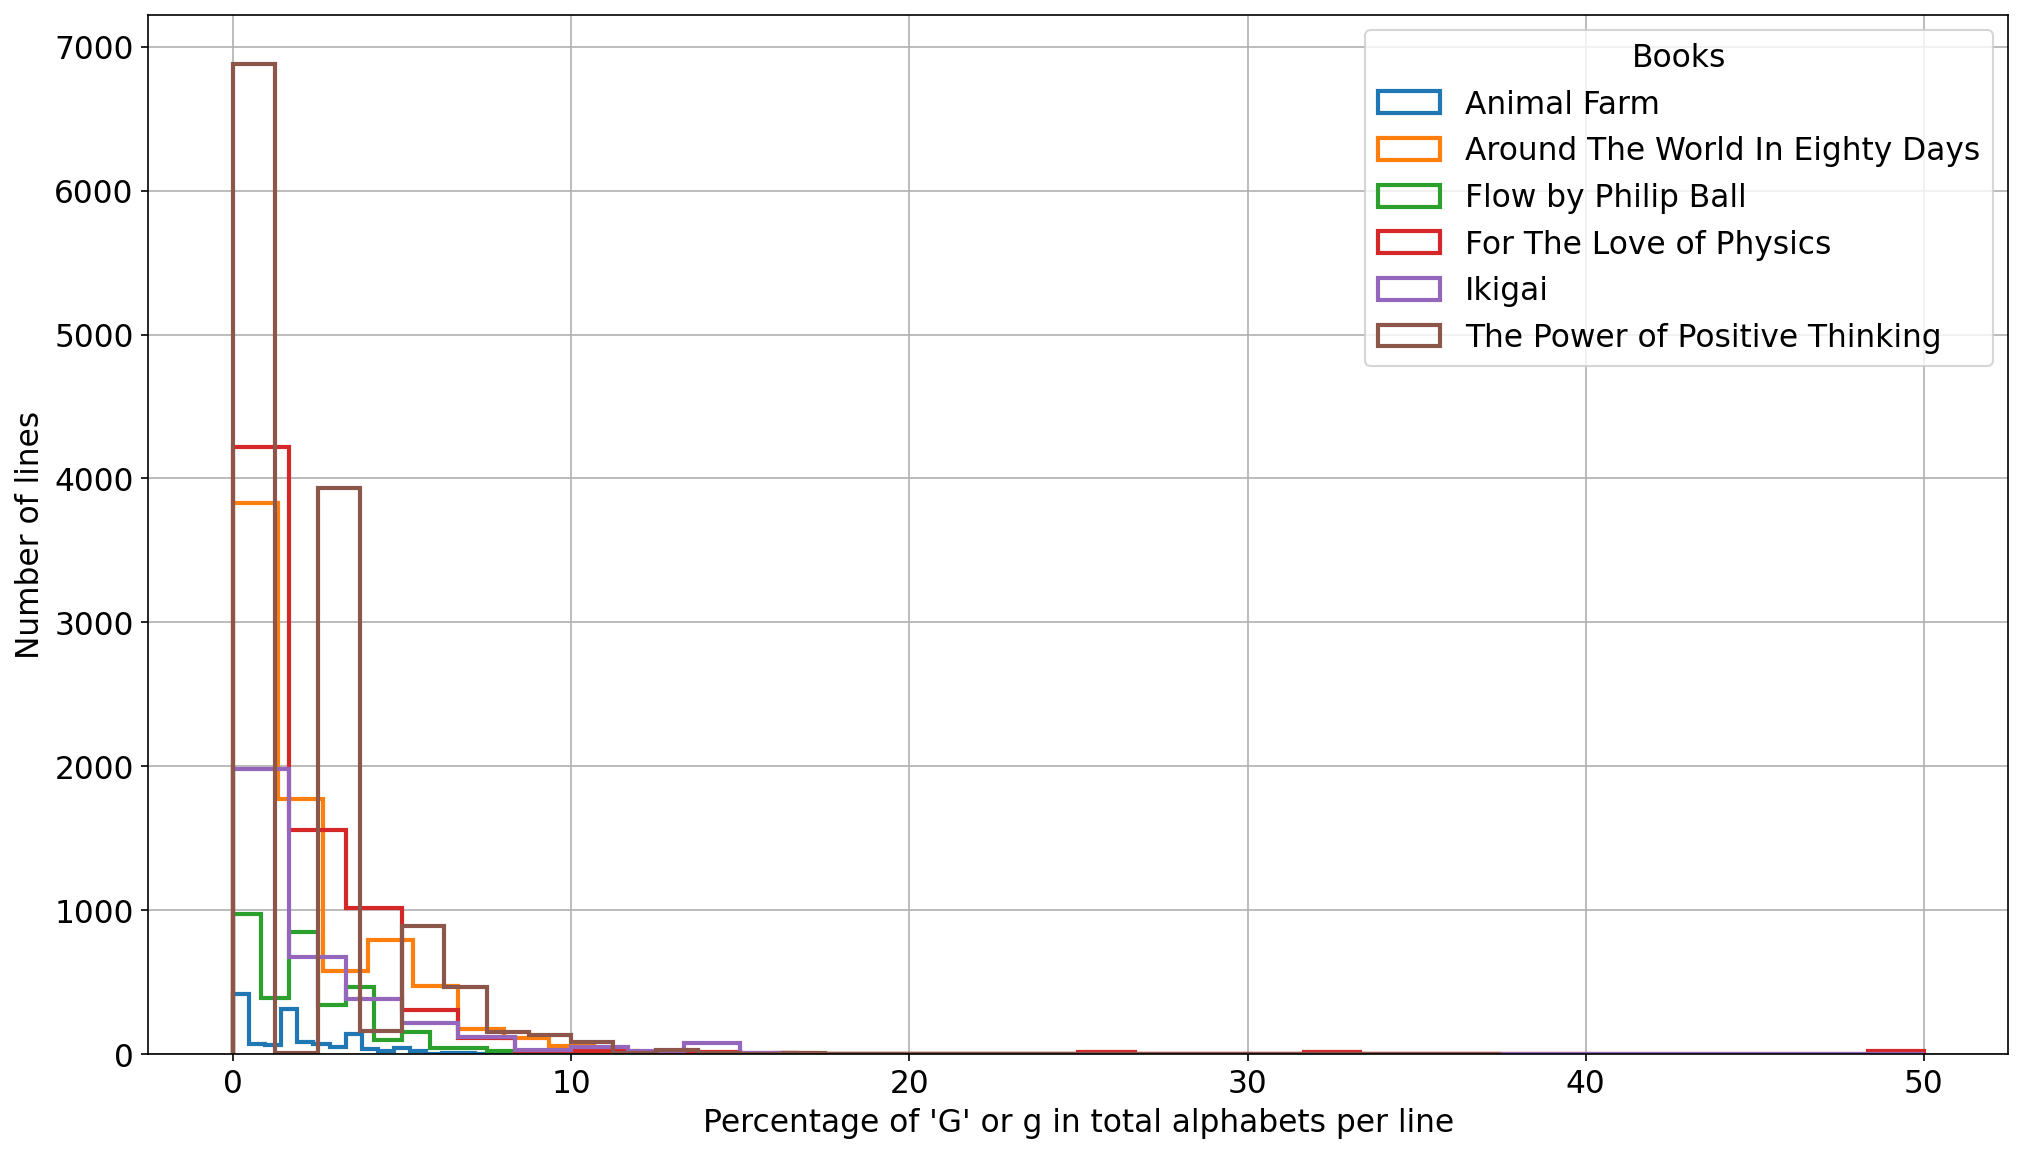
\includegraphics[scale=0.35]{../01_programFiles/histograms/g.png}\hspace{10ex}
    \end{center}
\end{frame}

\begin{frame}
    \frametitle{H or h}
    \begin{center}
        \hspace*{-5ex}
        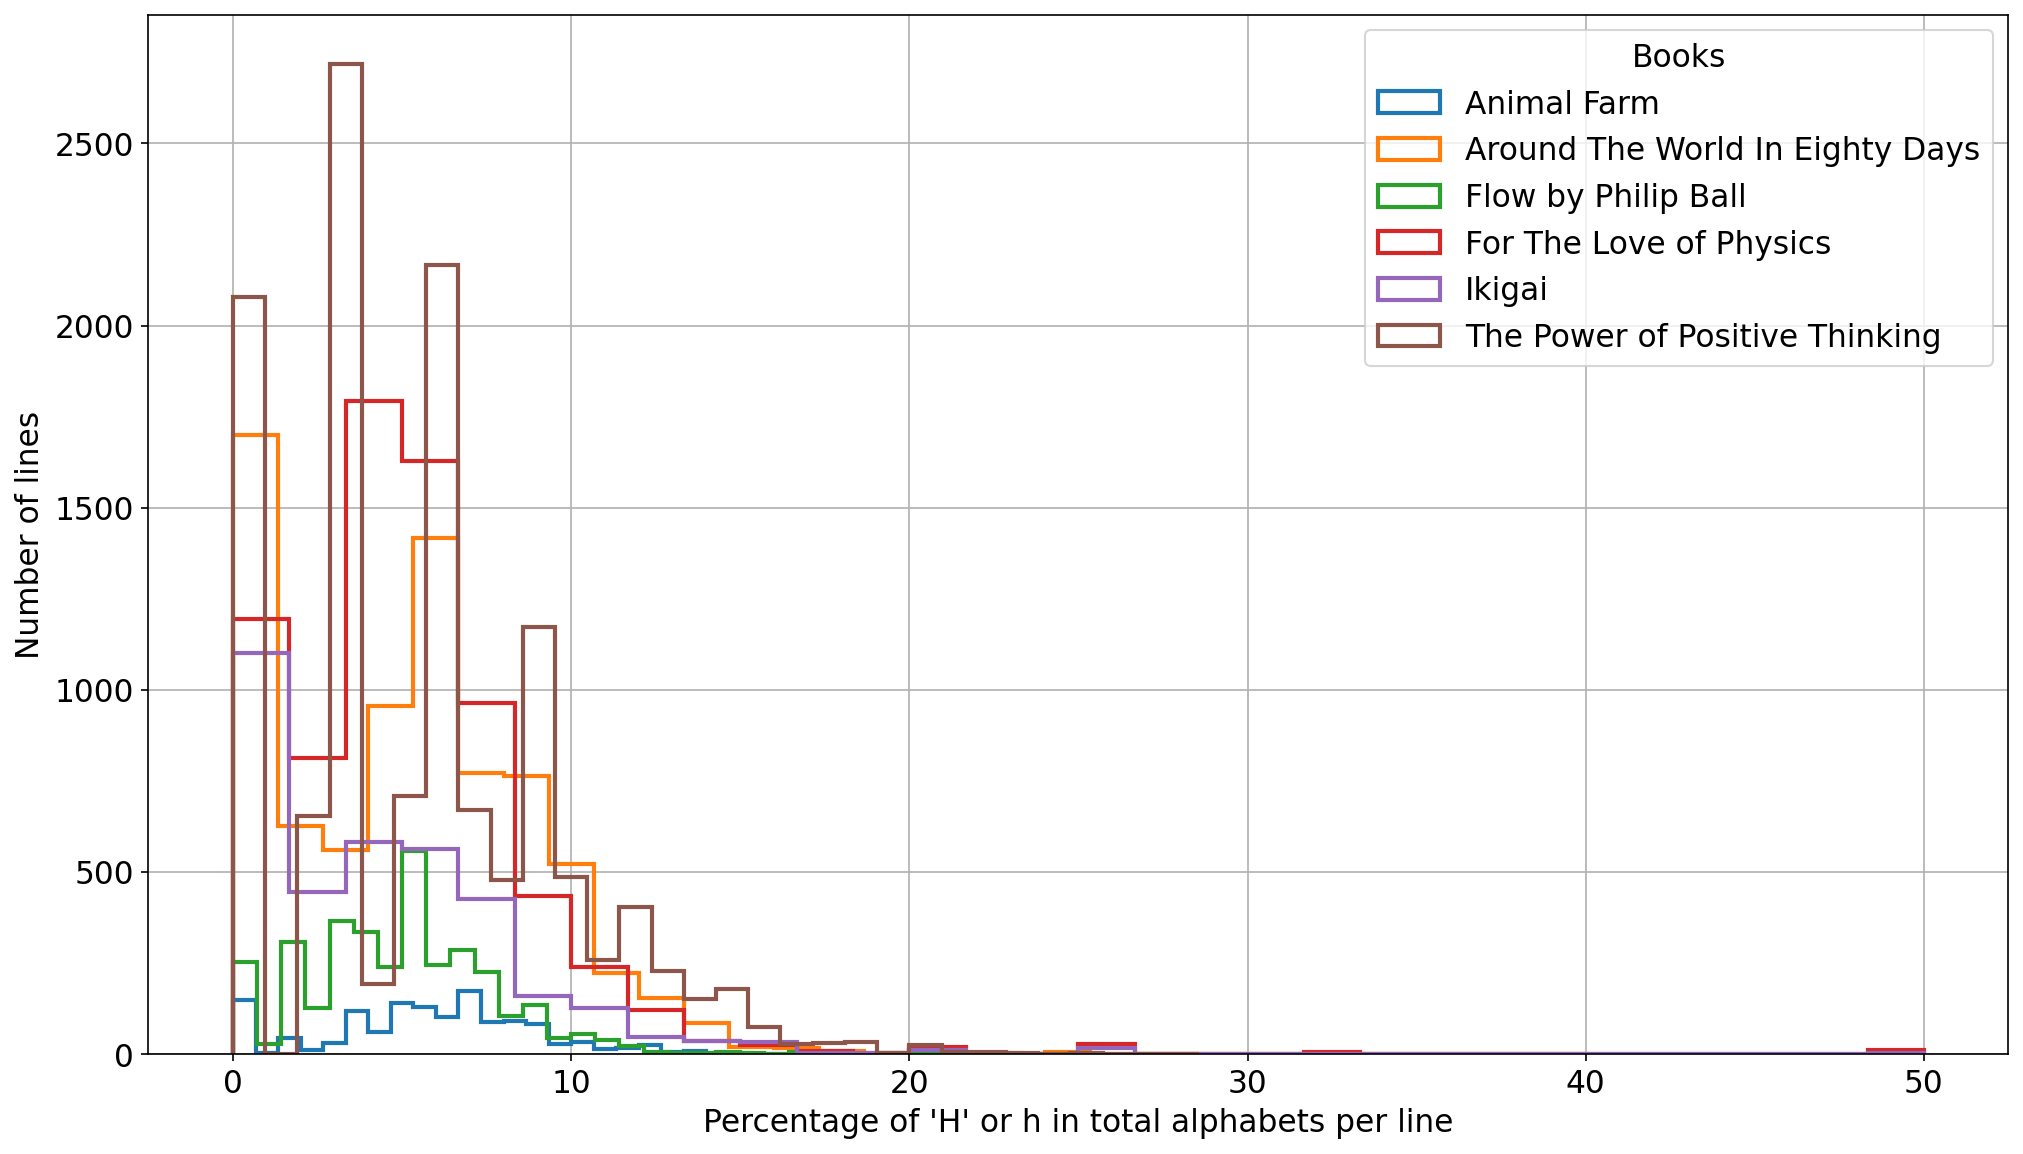
\includegraphics[scale=0.35]{../01_programFiles/histograms/h.png}\hspace{10ex}
    \end{center}
\end{frame}

\begin{frame}
    \frametitle{I or i}
    \begin{center}
        \hspace*{-5ex}
        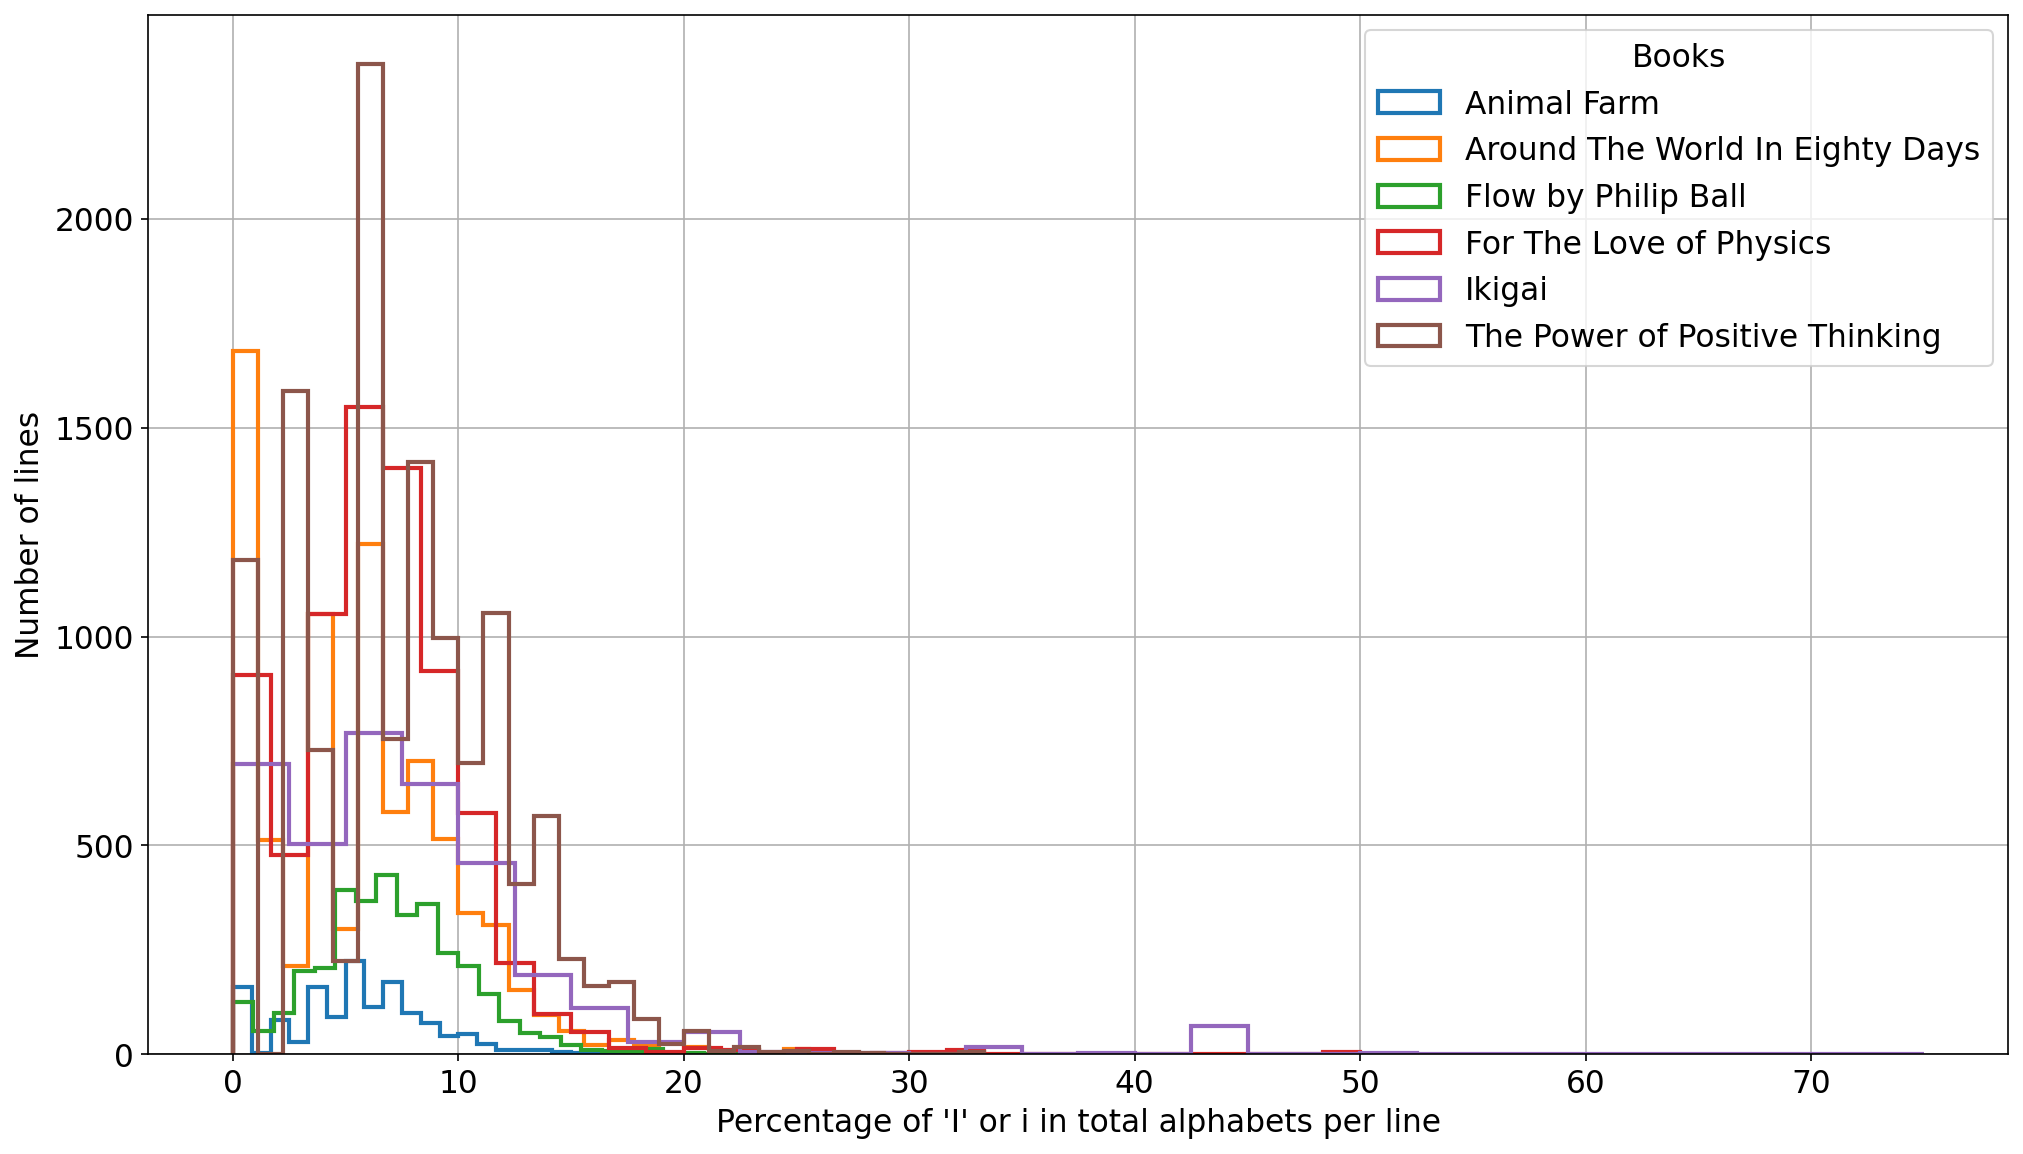
\includegraphics[scale=0.35]{../01_programFiles/histograms/i.png}\hspace{10ex}
    \end{center}
\end{frame}

\begin{frame}
    \frametitle{J or j}
    \begin{center}
        \hspace*{-5ex}
        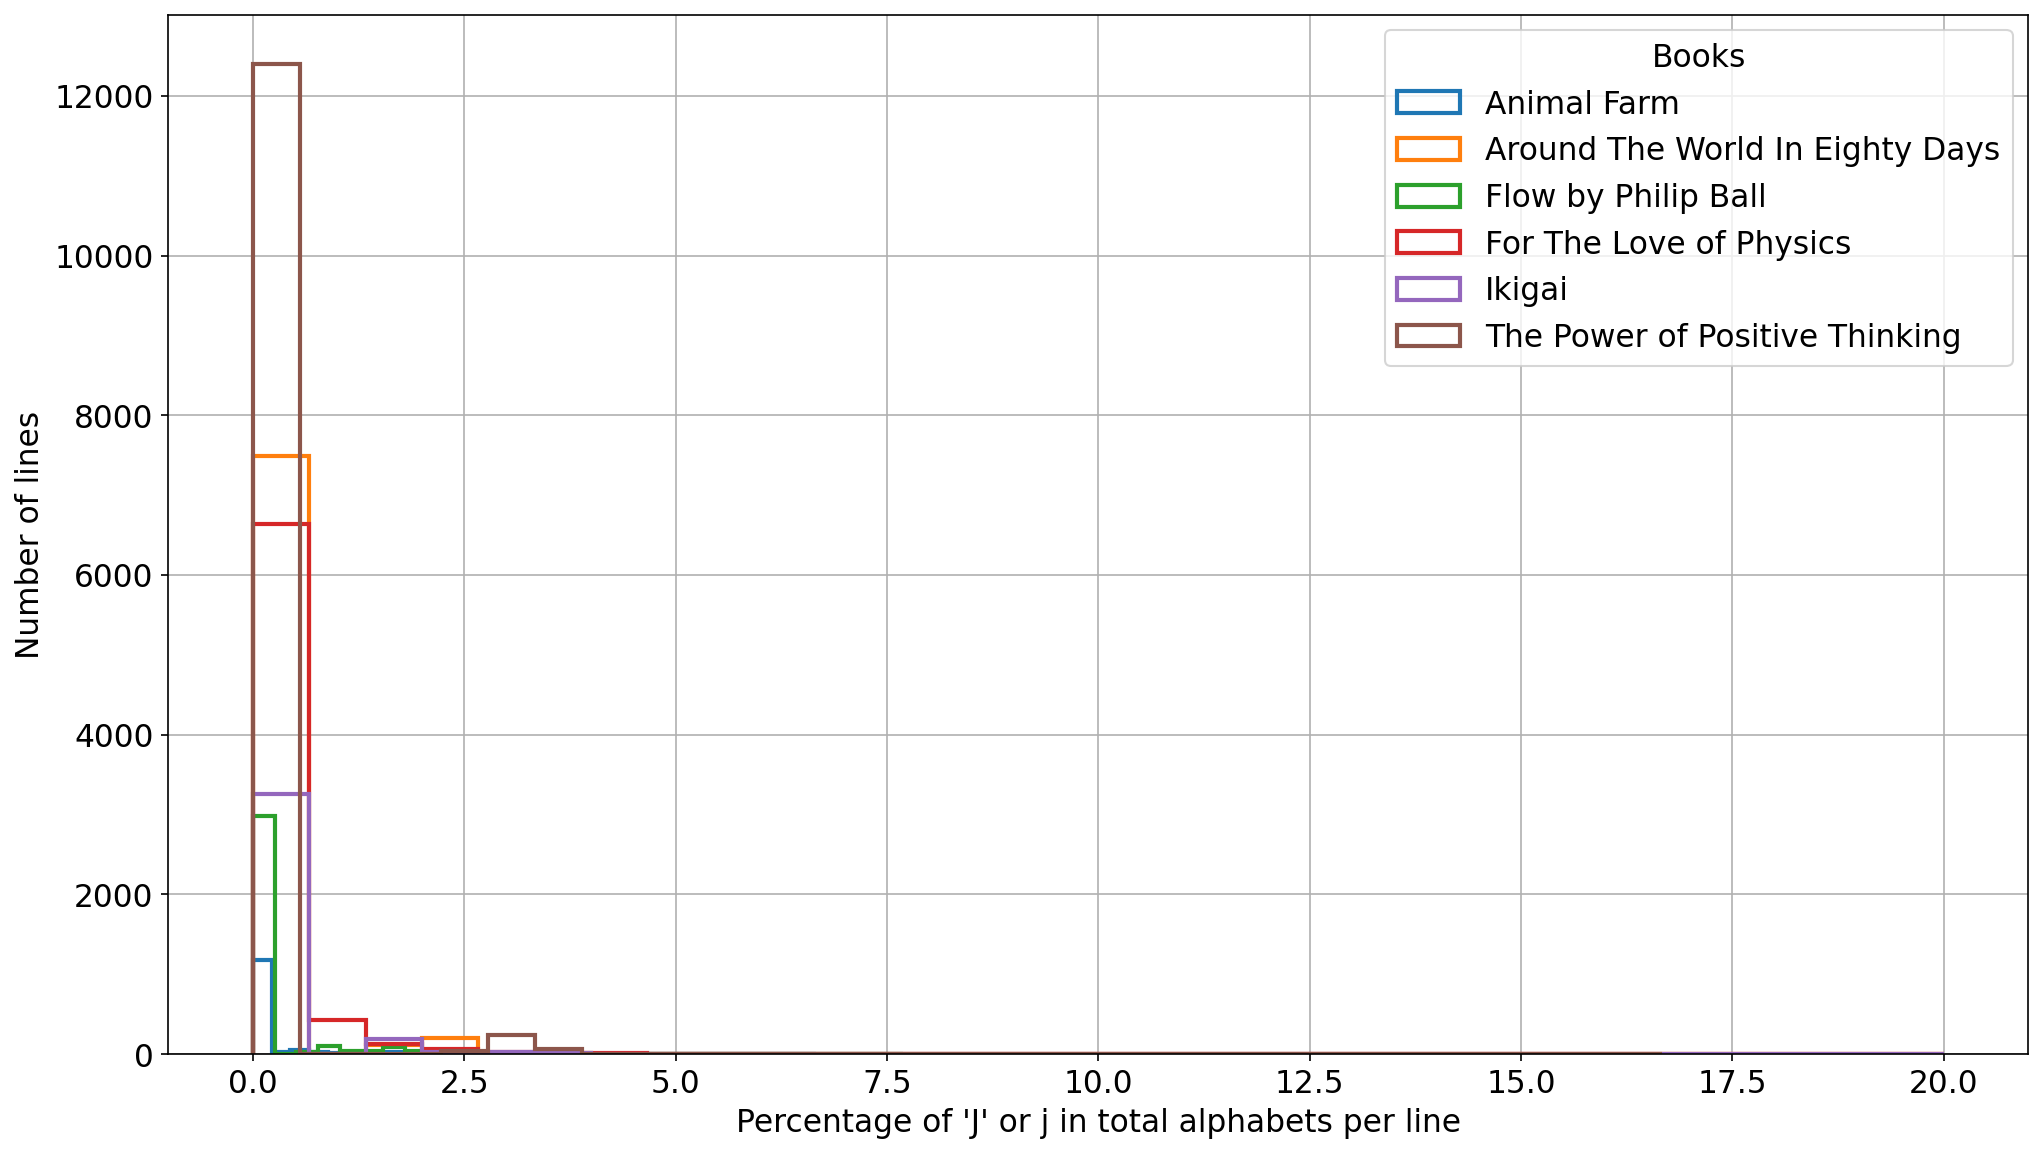
\includegraphics[scale=0.35]{../01_programFiles/histograms/j.png}\hspace{10ex}
    \end{center}
\end{frame}

\begin{frame}
    \frametitle{K or k}
    \begin{center}
        \hspace*{-5ex}
        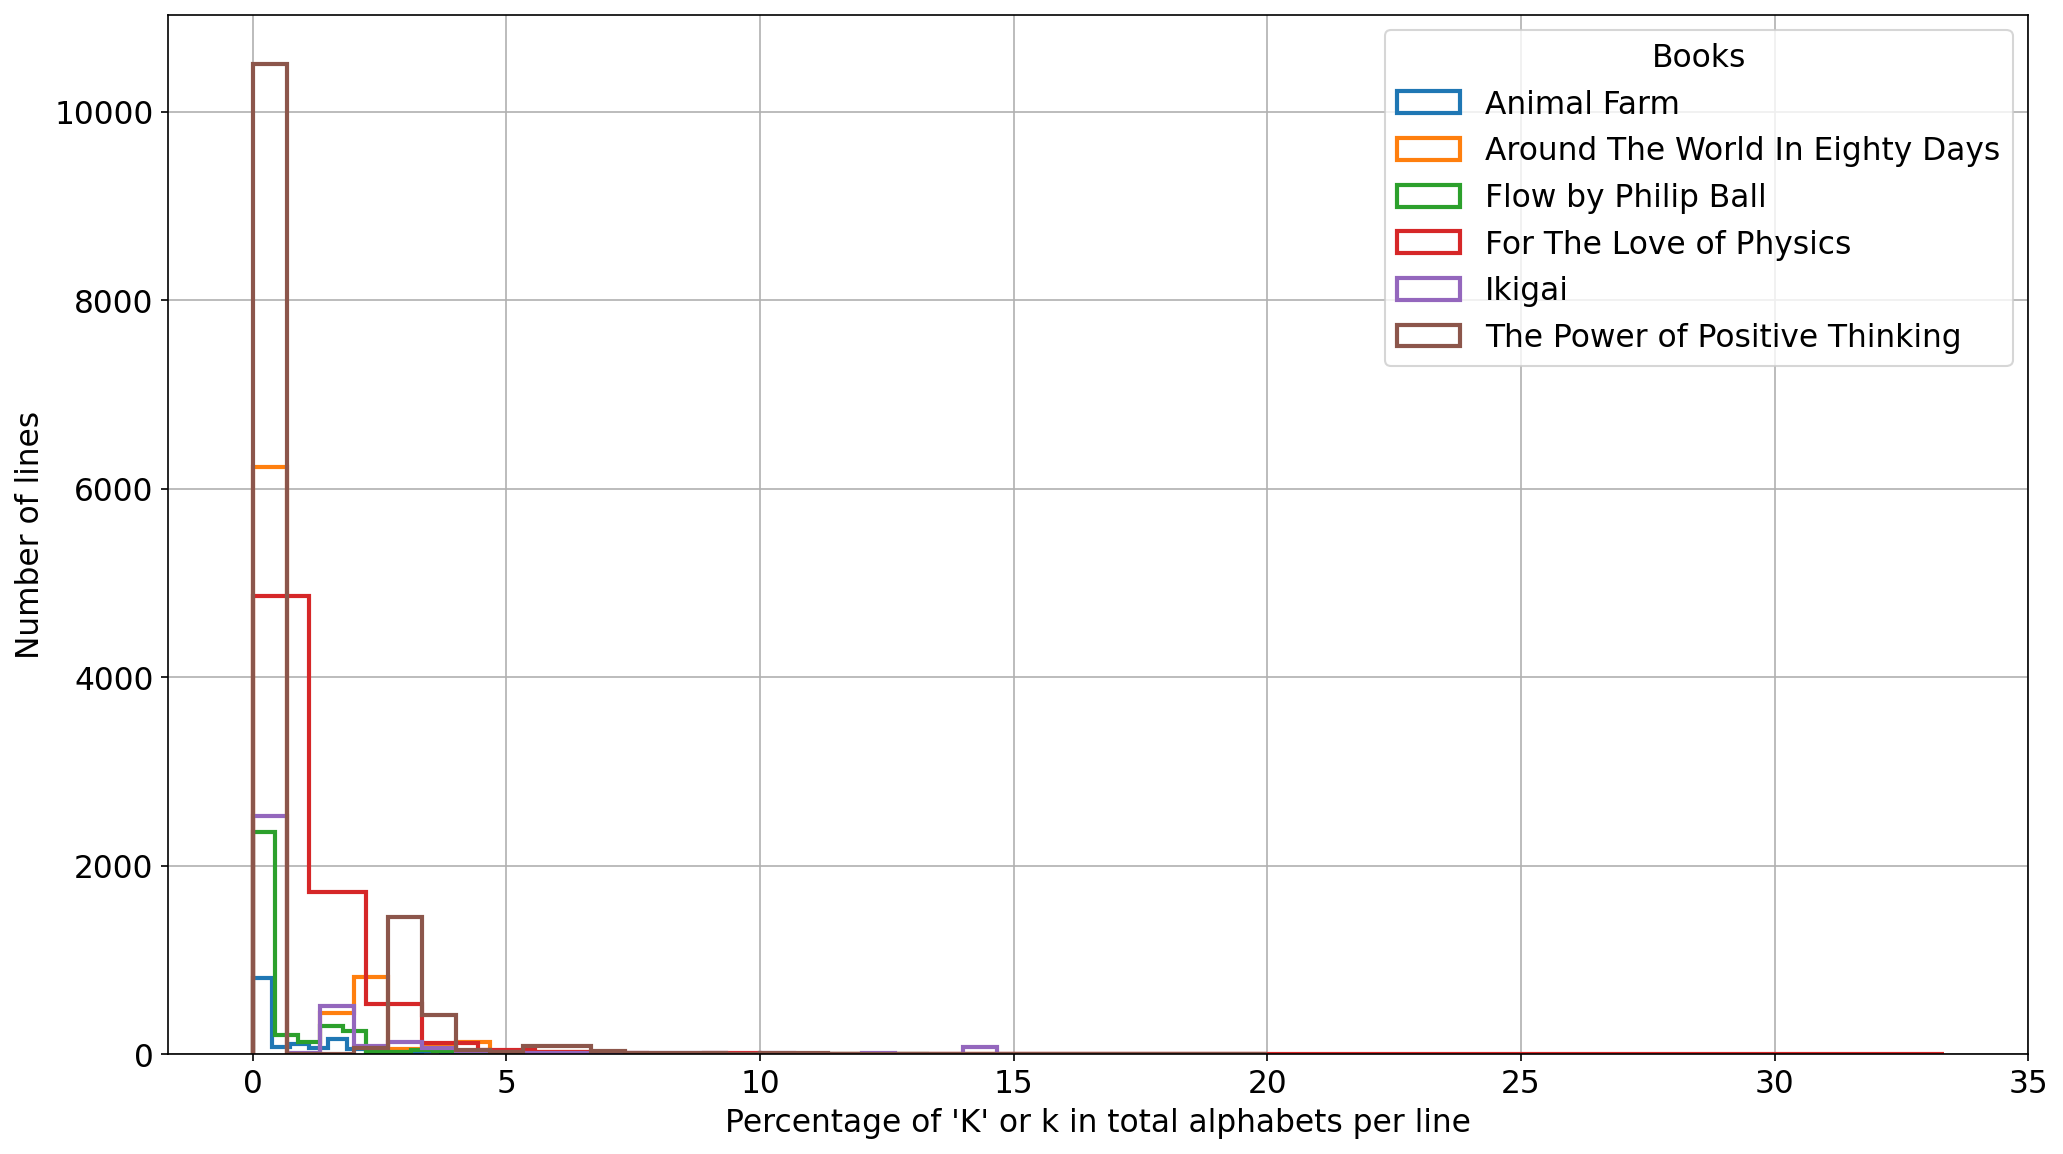
\includegraphics[scale=0.35]{../01_programFiles/histograms/k.png}\hspace{10ex}
    \end{center}
\end{frame}

\begin{frame}
    \frametitle{L or l}
    \begin{center}
        \hspace*{-5ex}
        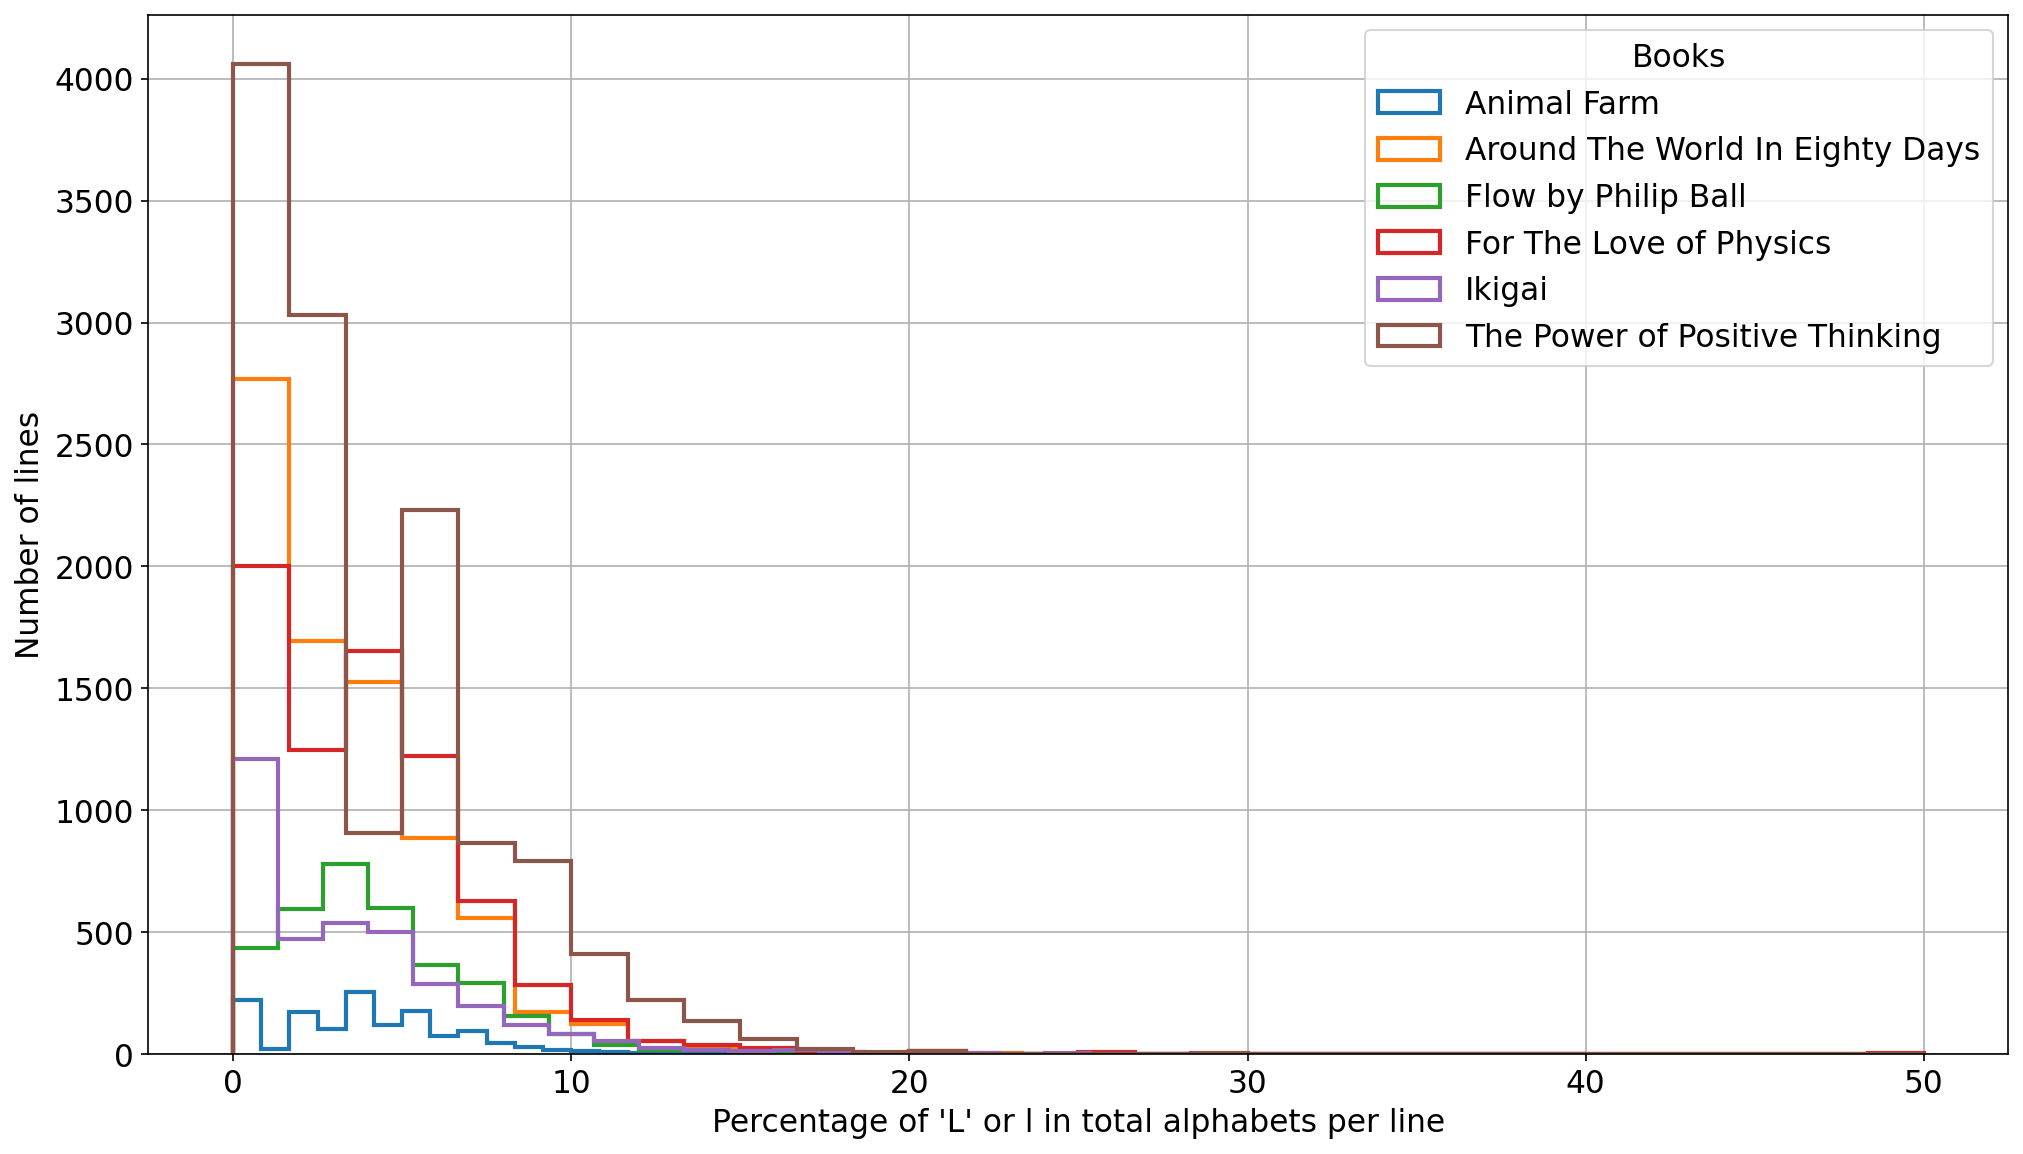
\includegraphics[scale=0.35]{../01_programFiles/histograms/l.png}\hspace{10ex}
    \end{center}
\end{frame}

\begin{frame}
    \frametitle{M or m}
    \begin{center}
        \hspace*{-5ex}
        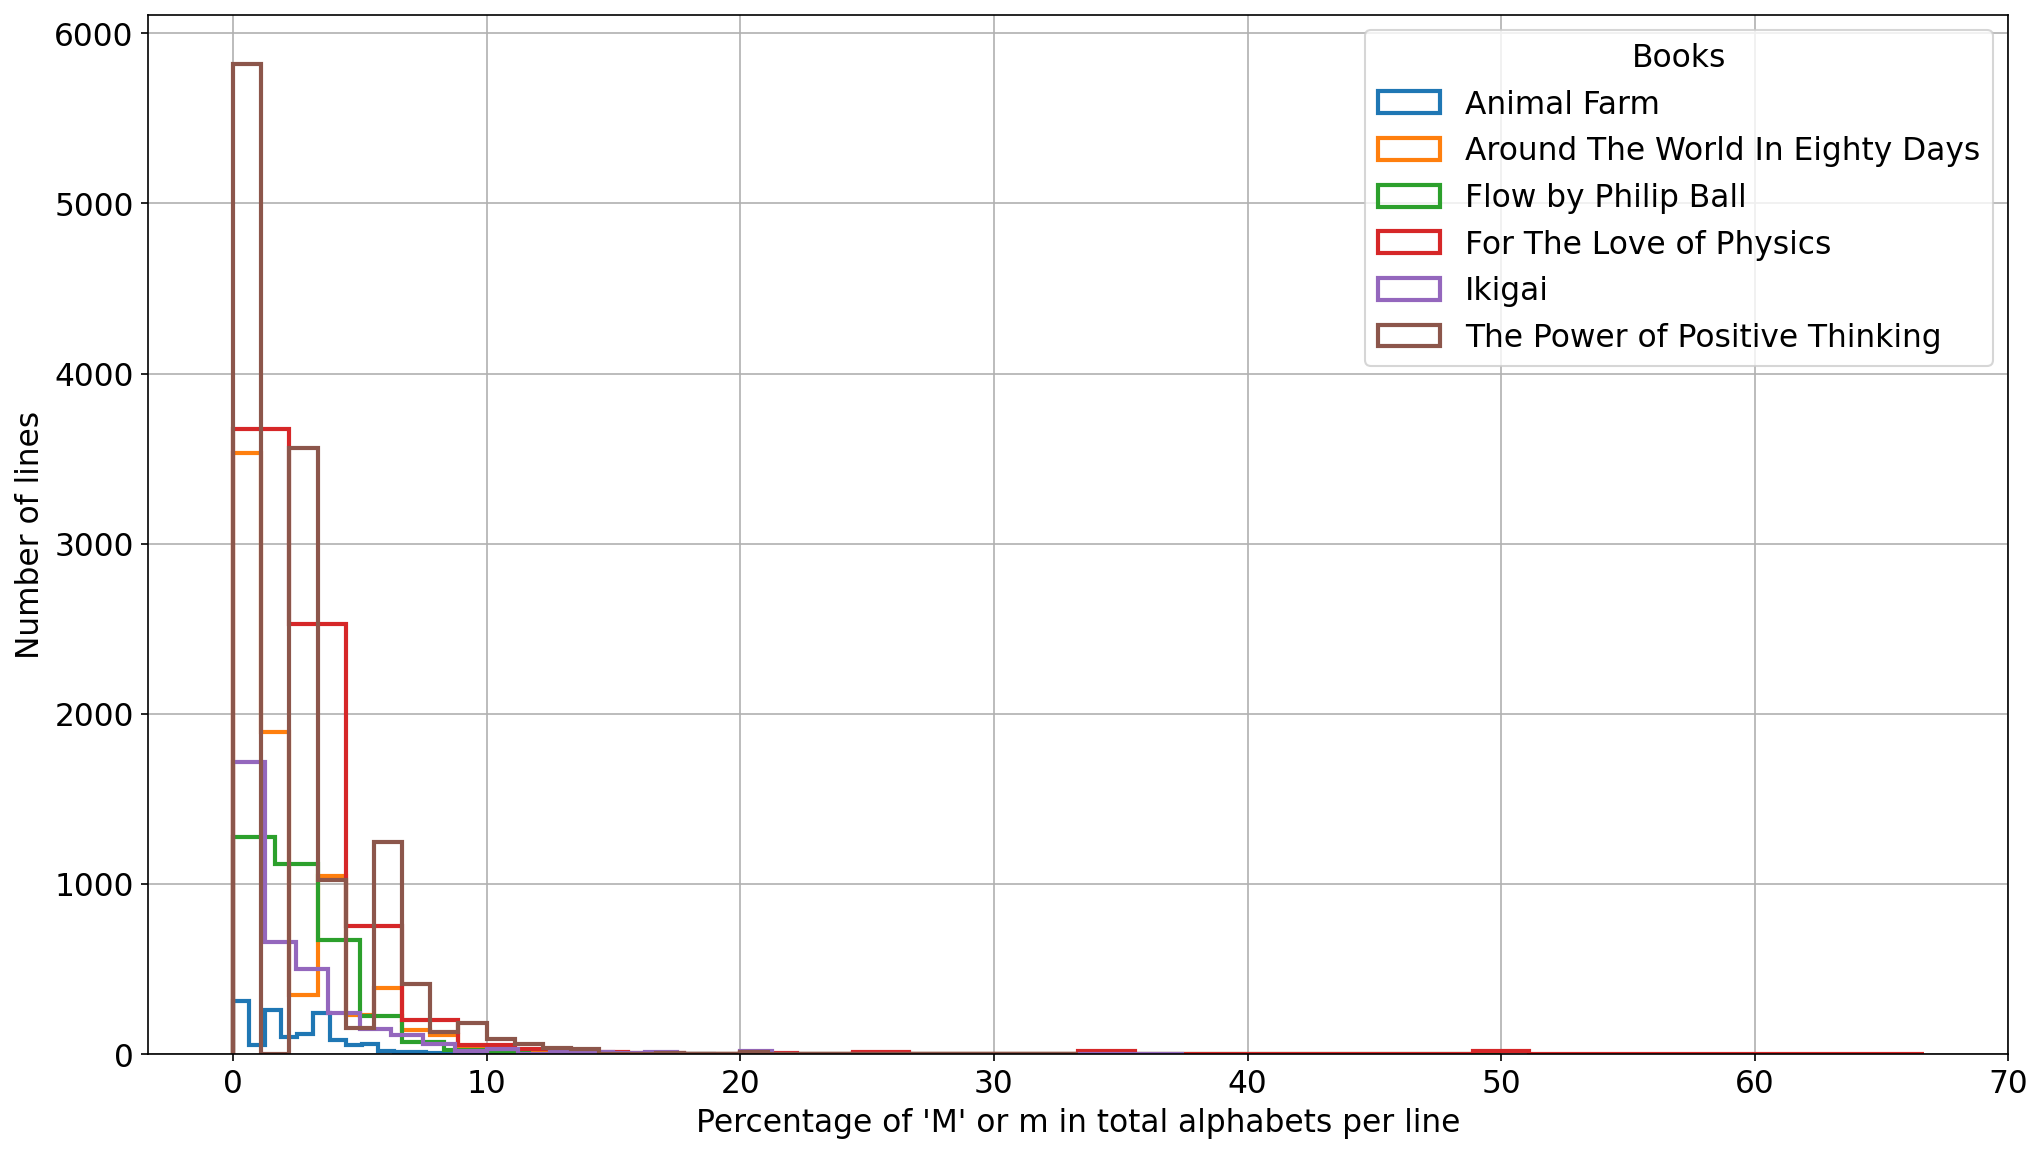
\includegraphics[scale=0.35]{../01_programFiles/histograms/m.png}\hspace{10ex}
    \end{center}
\end{frame}

\begin{frame}
    \frametitle{N or n}
    \begin{center}
        \hspace*{-5ex}
        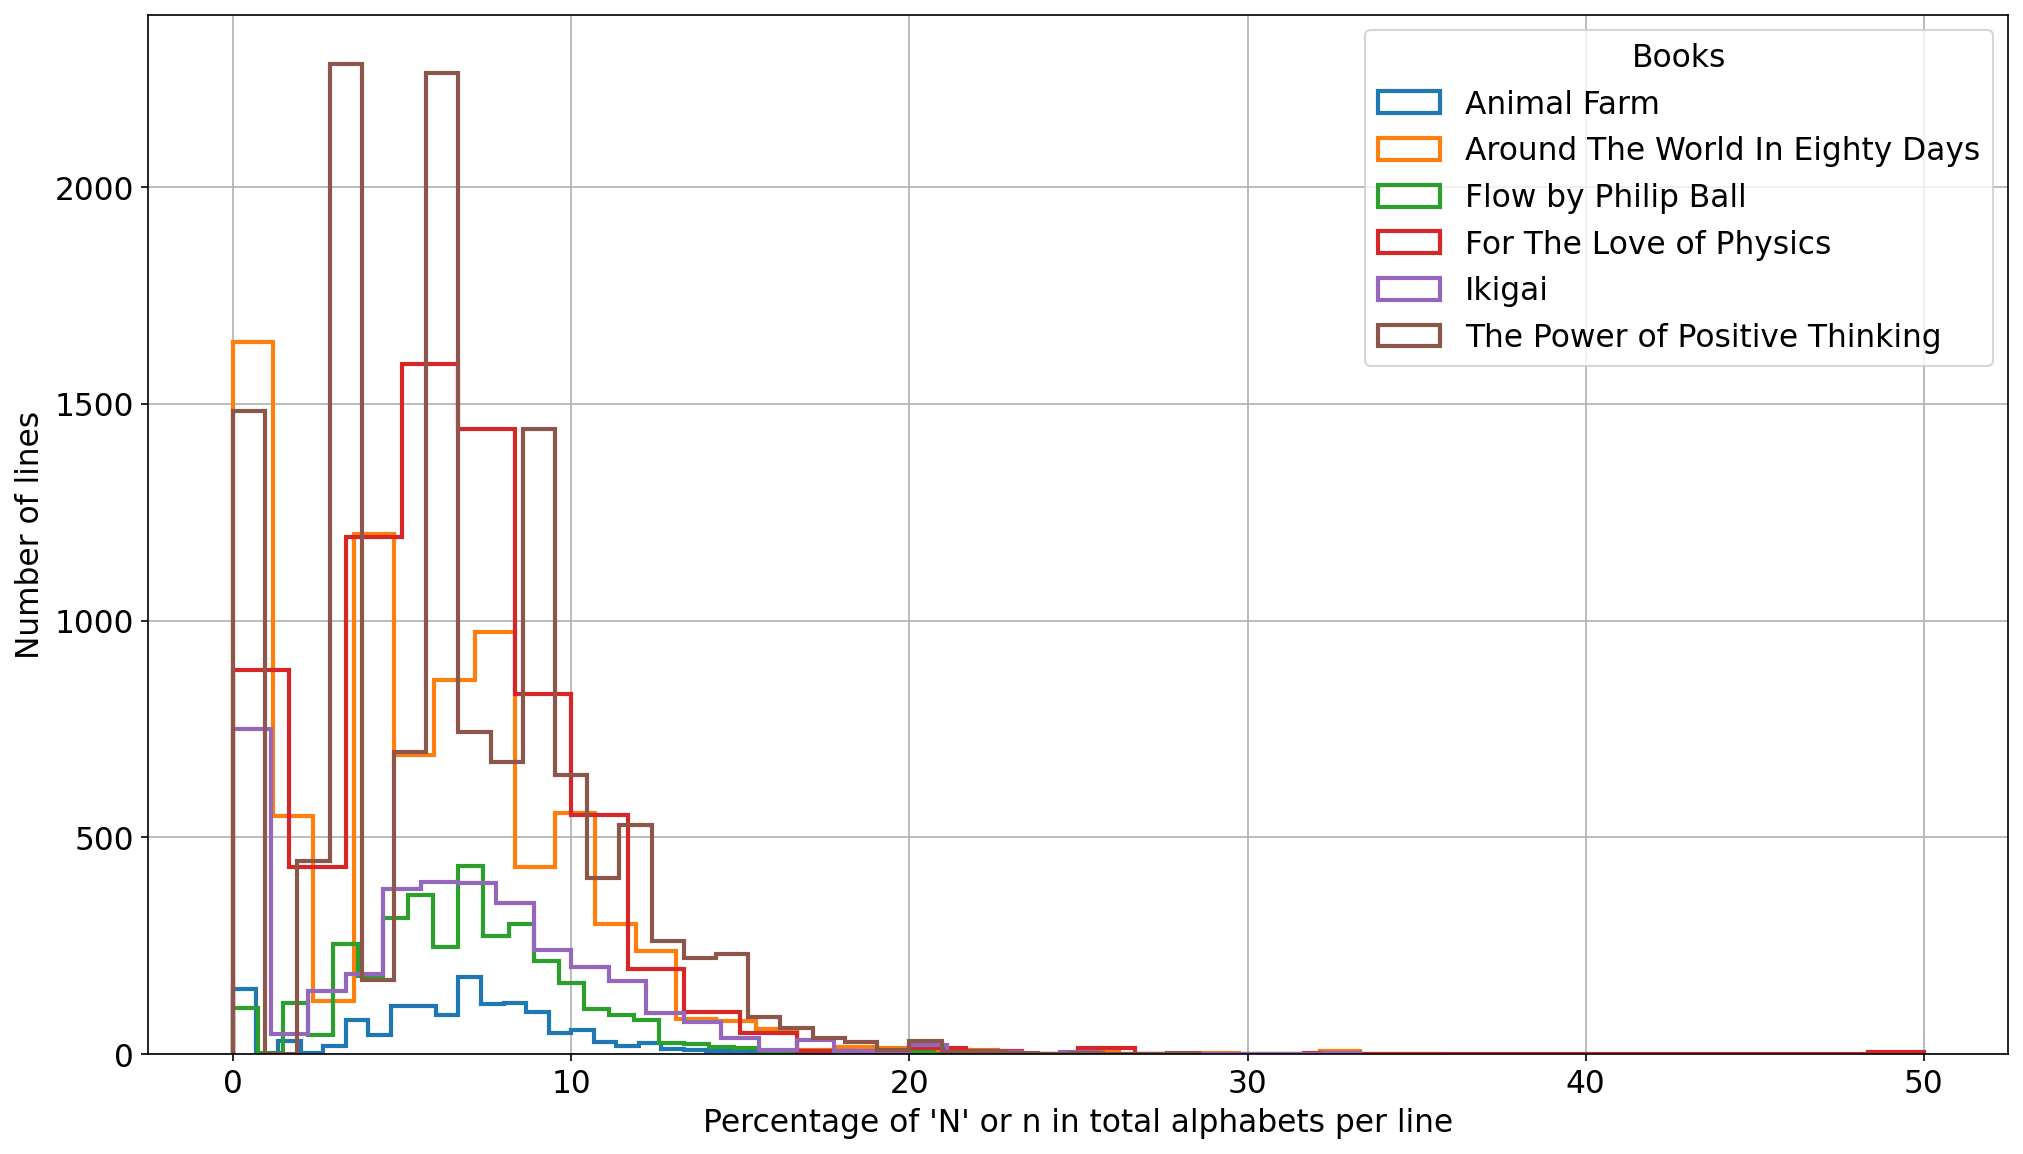
\includegraphics[scale=0.35]{../01_programFiles/histograms/n.png}\hspace{10ex}
    \end{center}
\end{frame}

\begin{frame}
    \frametitle{O or o}
    \begin{center}
        \hspace*{-5ex}
        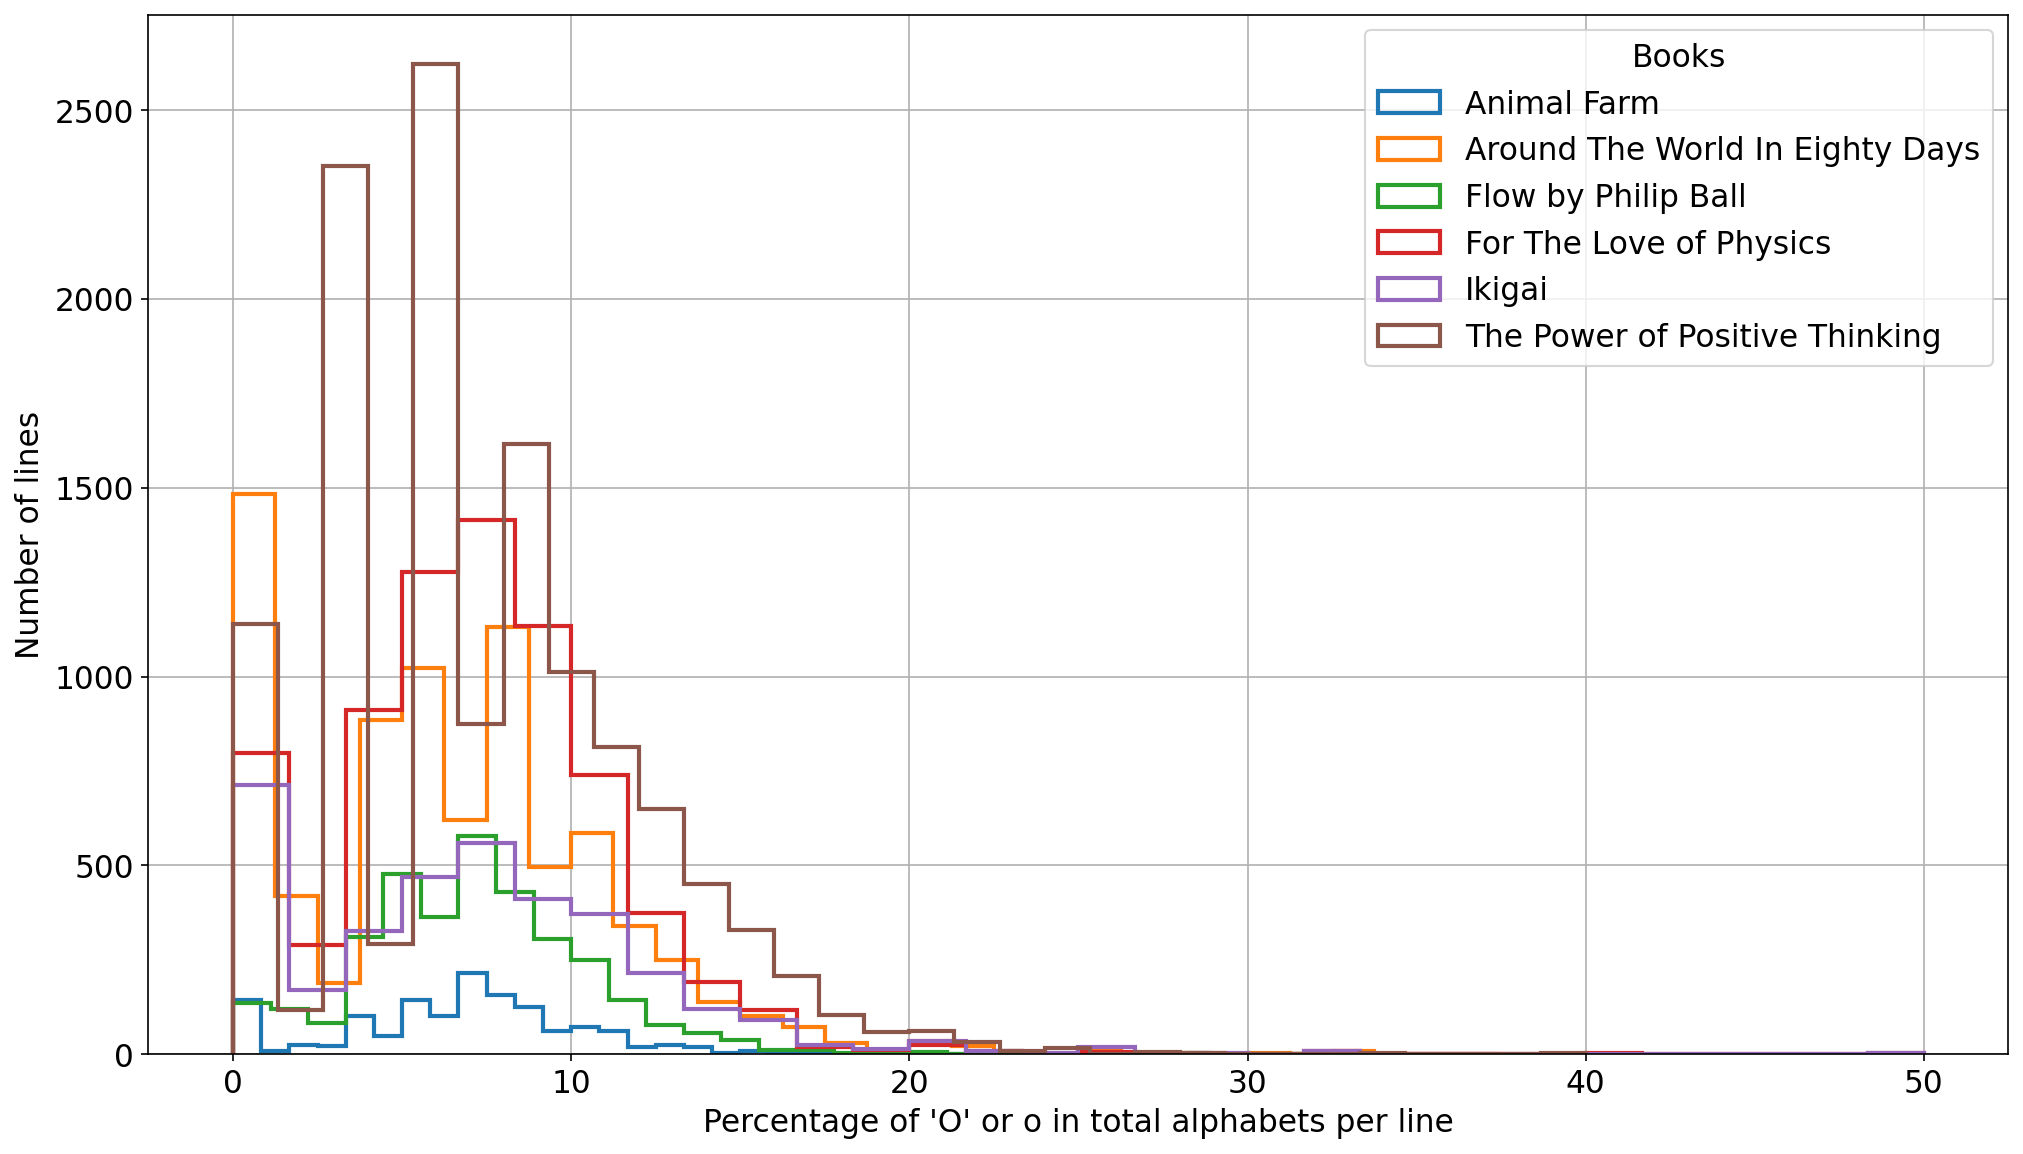
\includegraphics[scale=0.35]{../01_programFiles/histograms/o.png}\hspace{10ex}
    \end{center}
\end{frame}

\begin{frame}
    \frametitle{P or p}
    \begin{center}
        \hspace*{-5ex}
        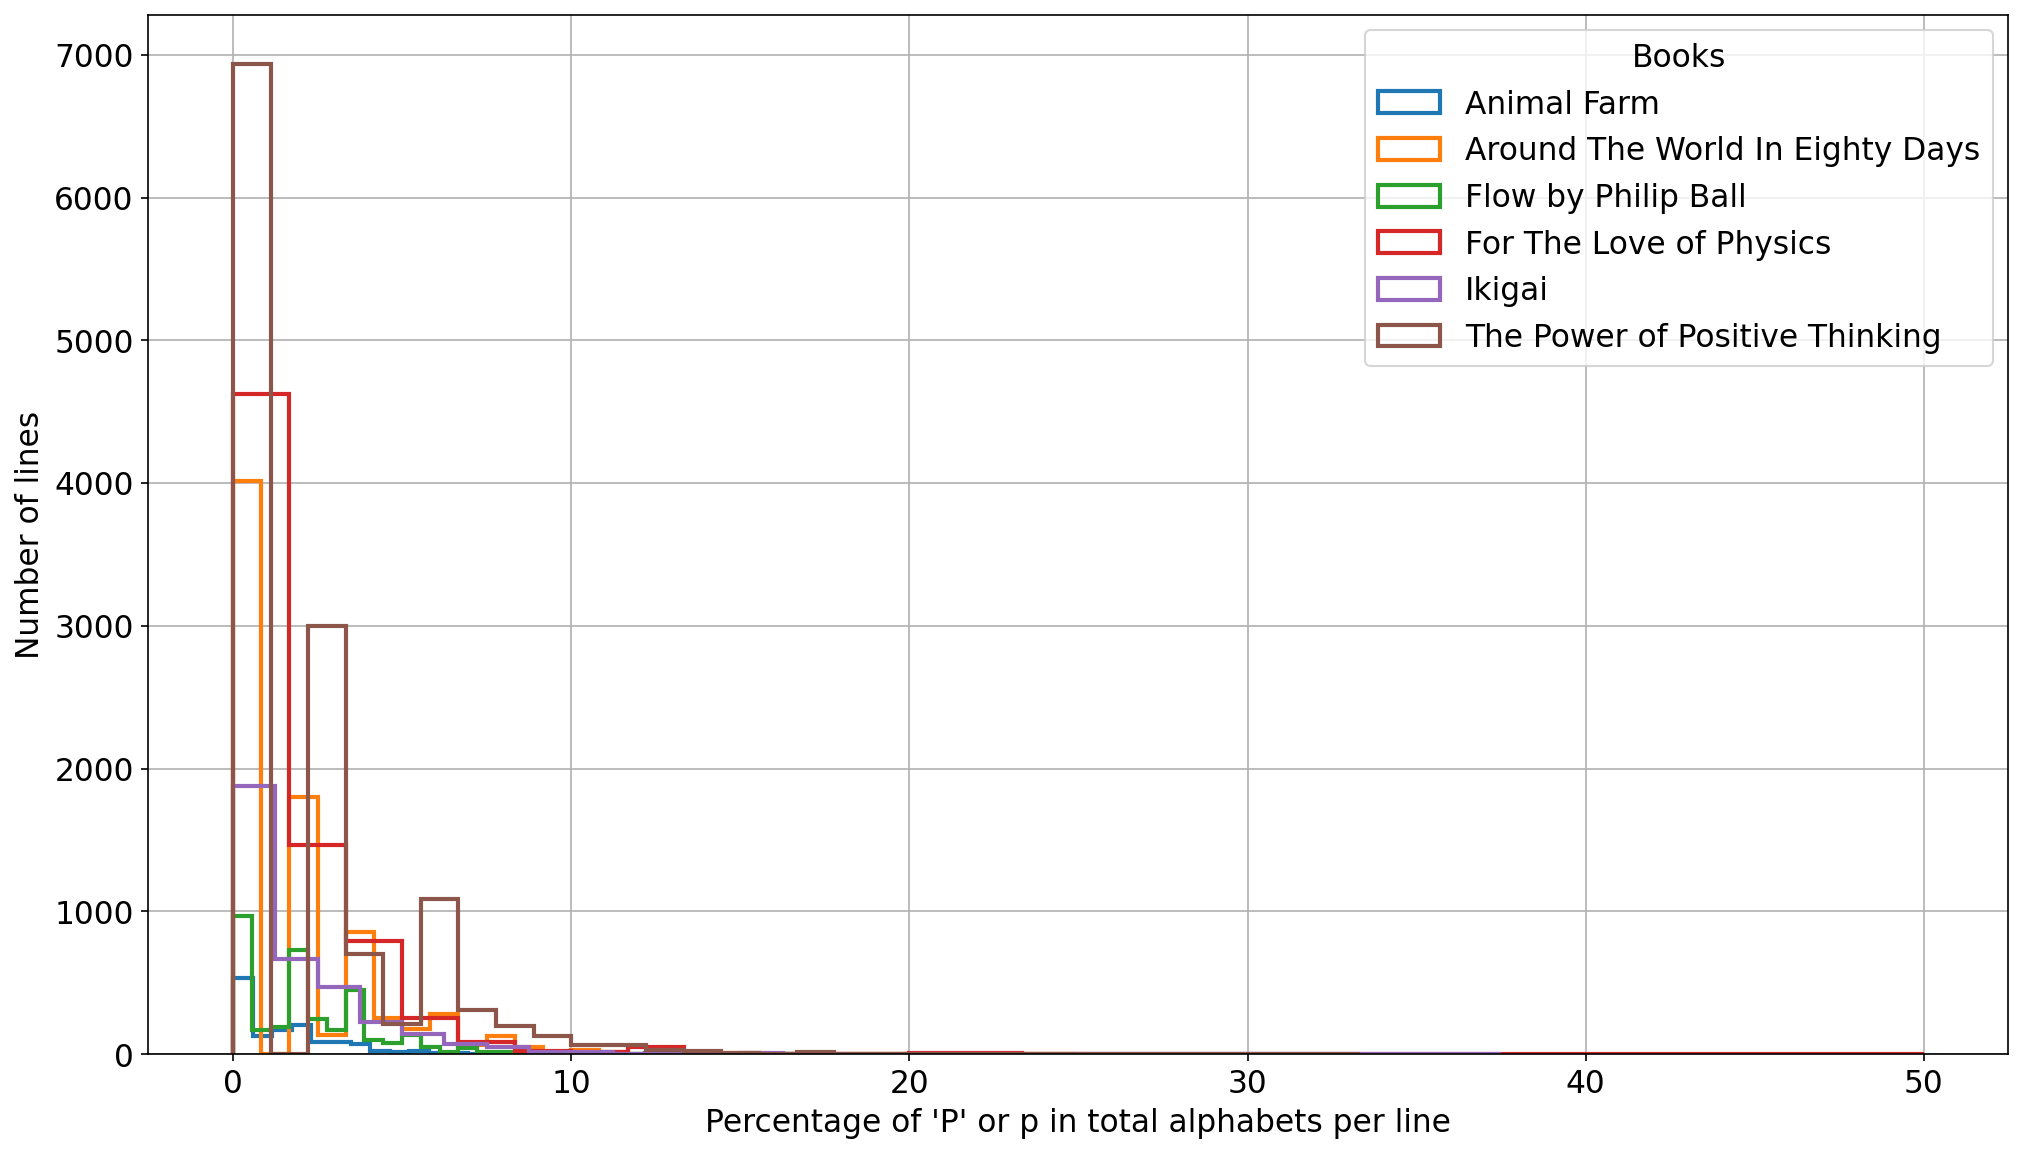
\includegraphics[scale=0.35]{../01_programFiles/histograms/p.png}\hspace{10ex}
    \end{center}
\end{frame}

\begin{frame}
    \frametitle{Q or q}
    \begin{center}
        \hspace*{-5ex}
        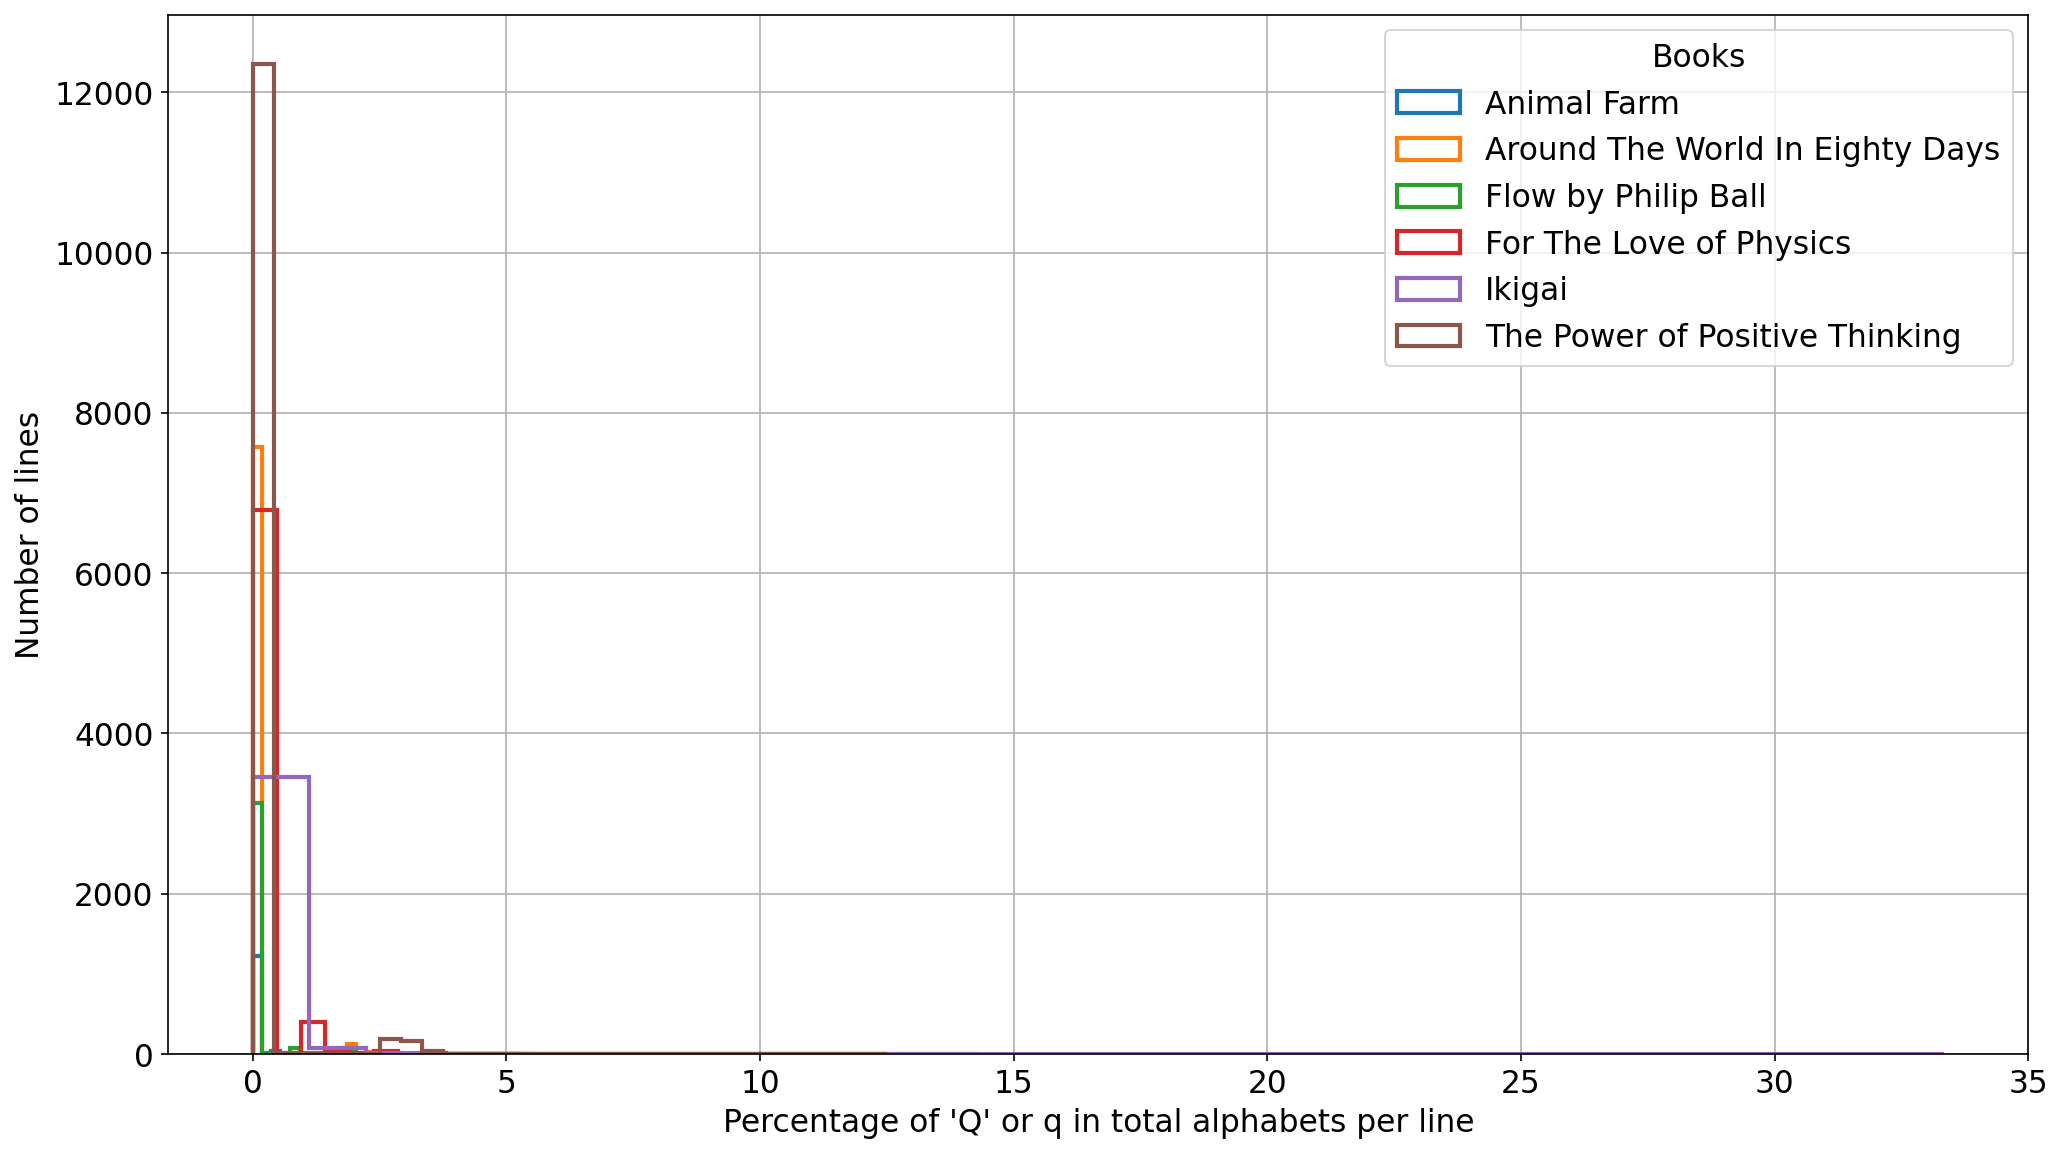
\includegraphics[scale=0.35]{../01_programFiles/histograms/q.png}\hspace{10ex}
    \end{center}
\end{frame}

\begin{frame}
    \frametitle{R or r}
    \begin{center}
        \hspace*{-5ex}
        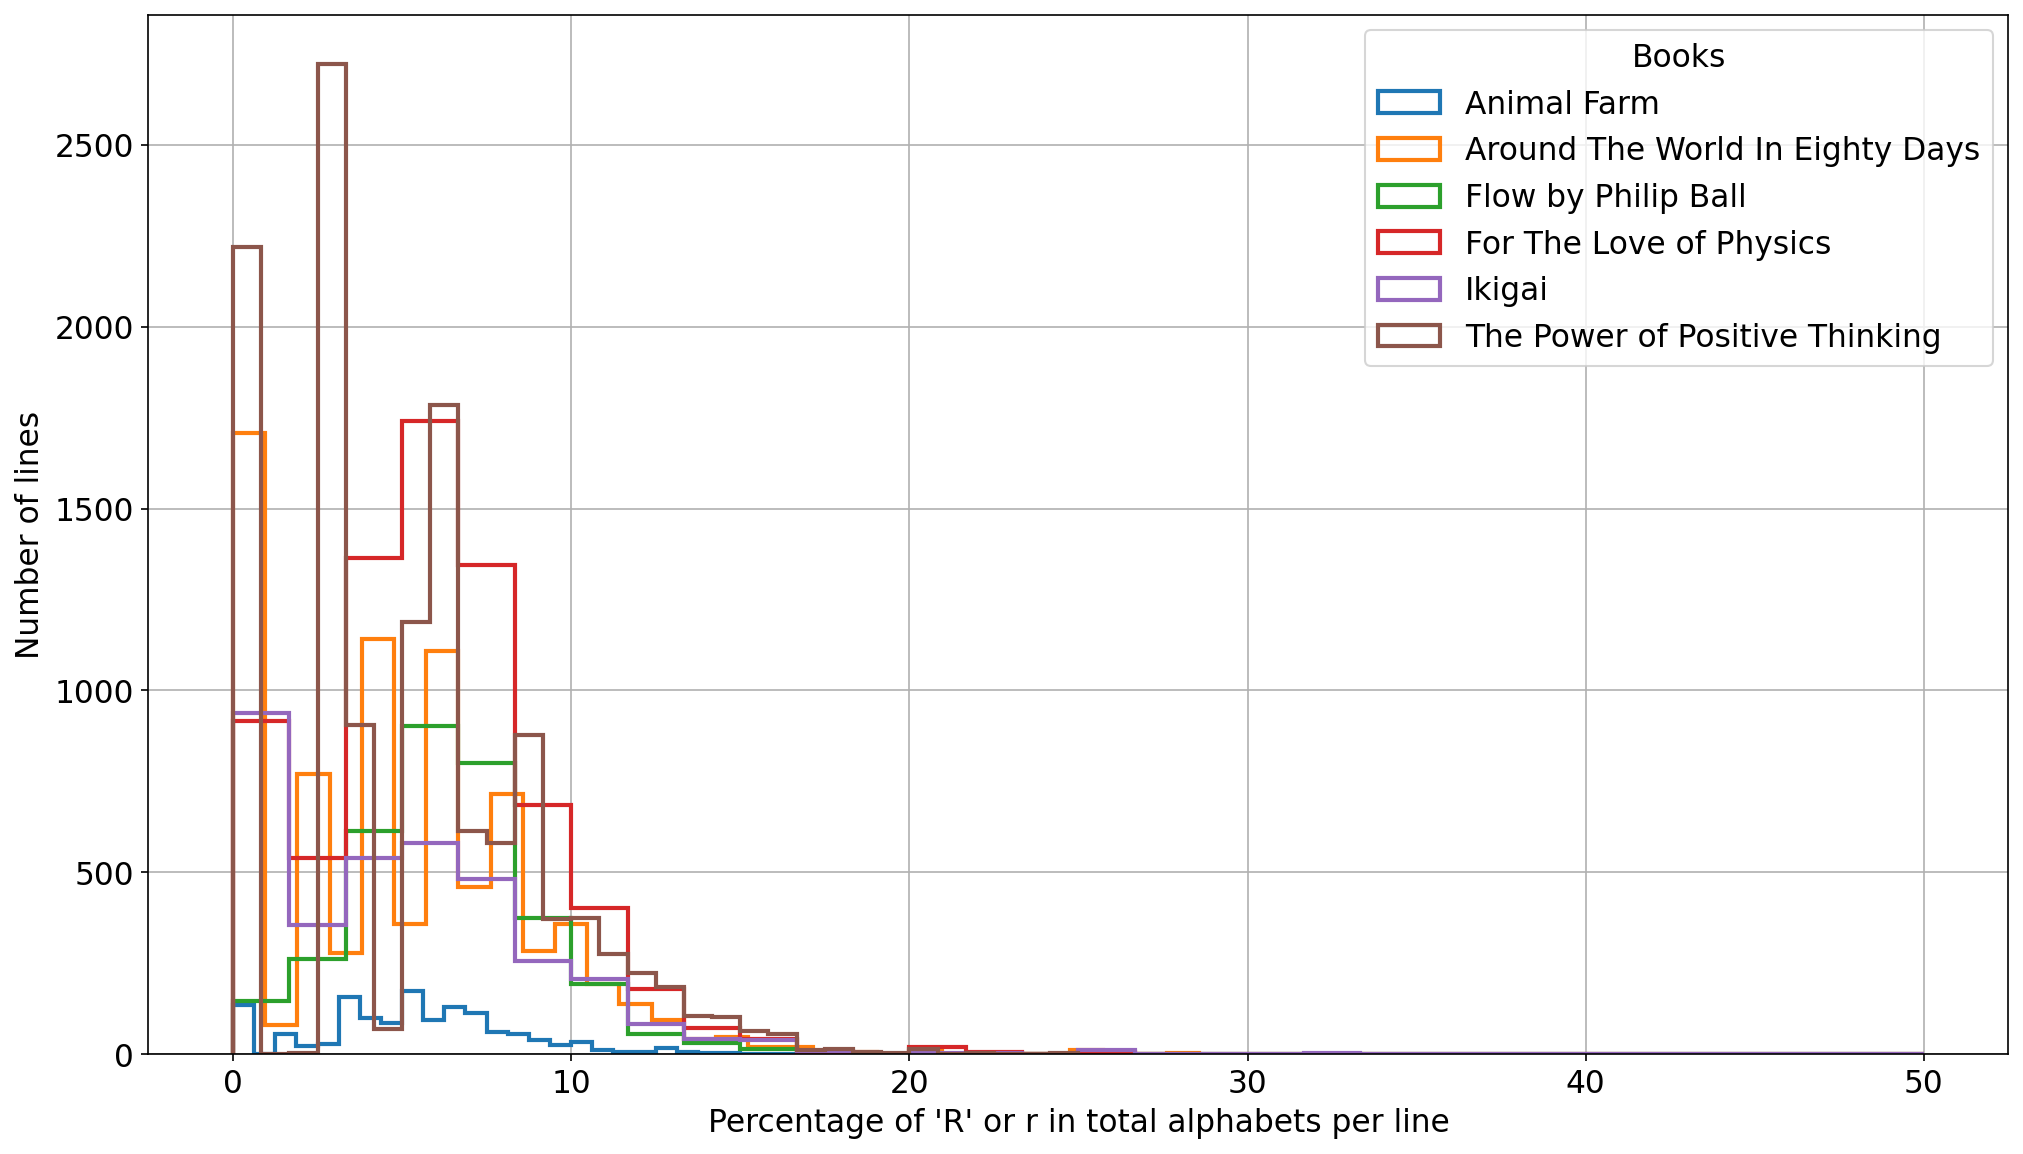
\includegraphics[scale=0.35]{../01_programFiles/histograms/r.png}\hspace{10ex}
    \end{center}
\end{frame}

\begin{frame}
    \frametitle{S or s}
    \begin{center}
        \hspace*{-5ex}
        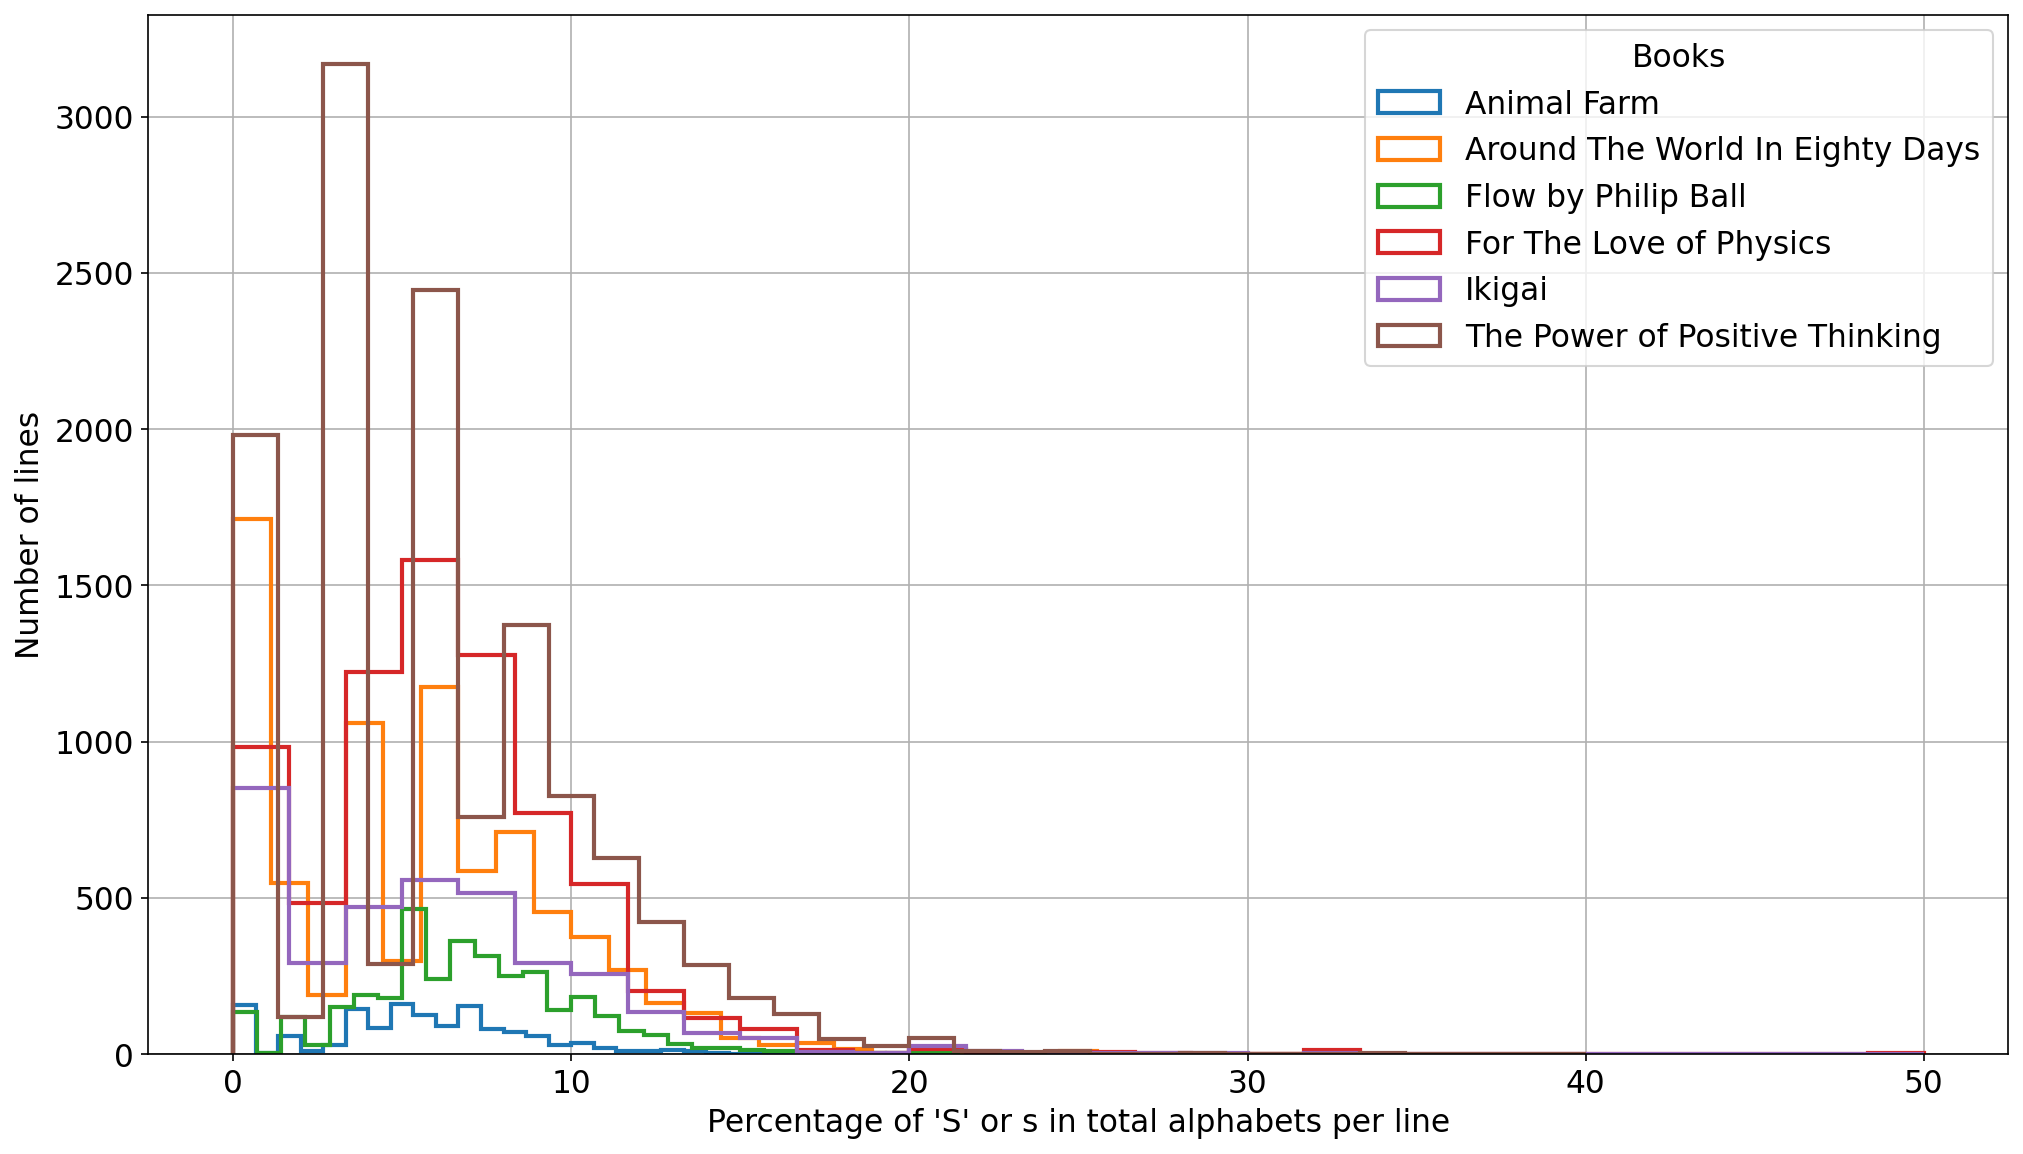
\includegraphics[scale=0.35]{../01_programFiles/histograms/s.png}\hspace{10ex}
    \end{center}
\end{frame}

\begin{frame}
    \frametitle{T or t}
    \begin{center}
        \hspace*{-5ex}
        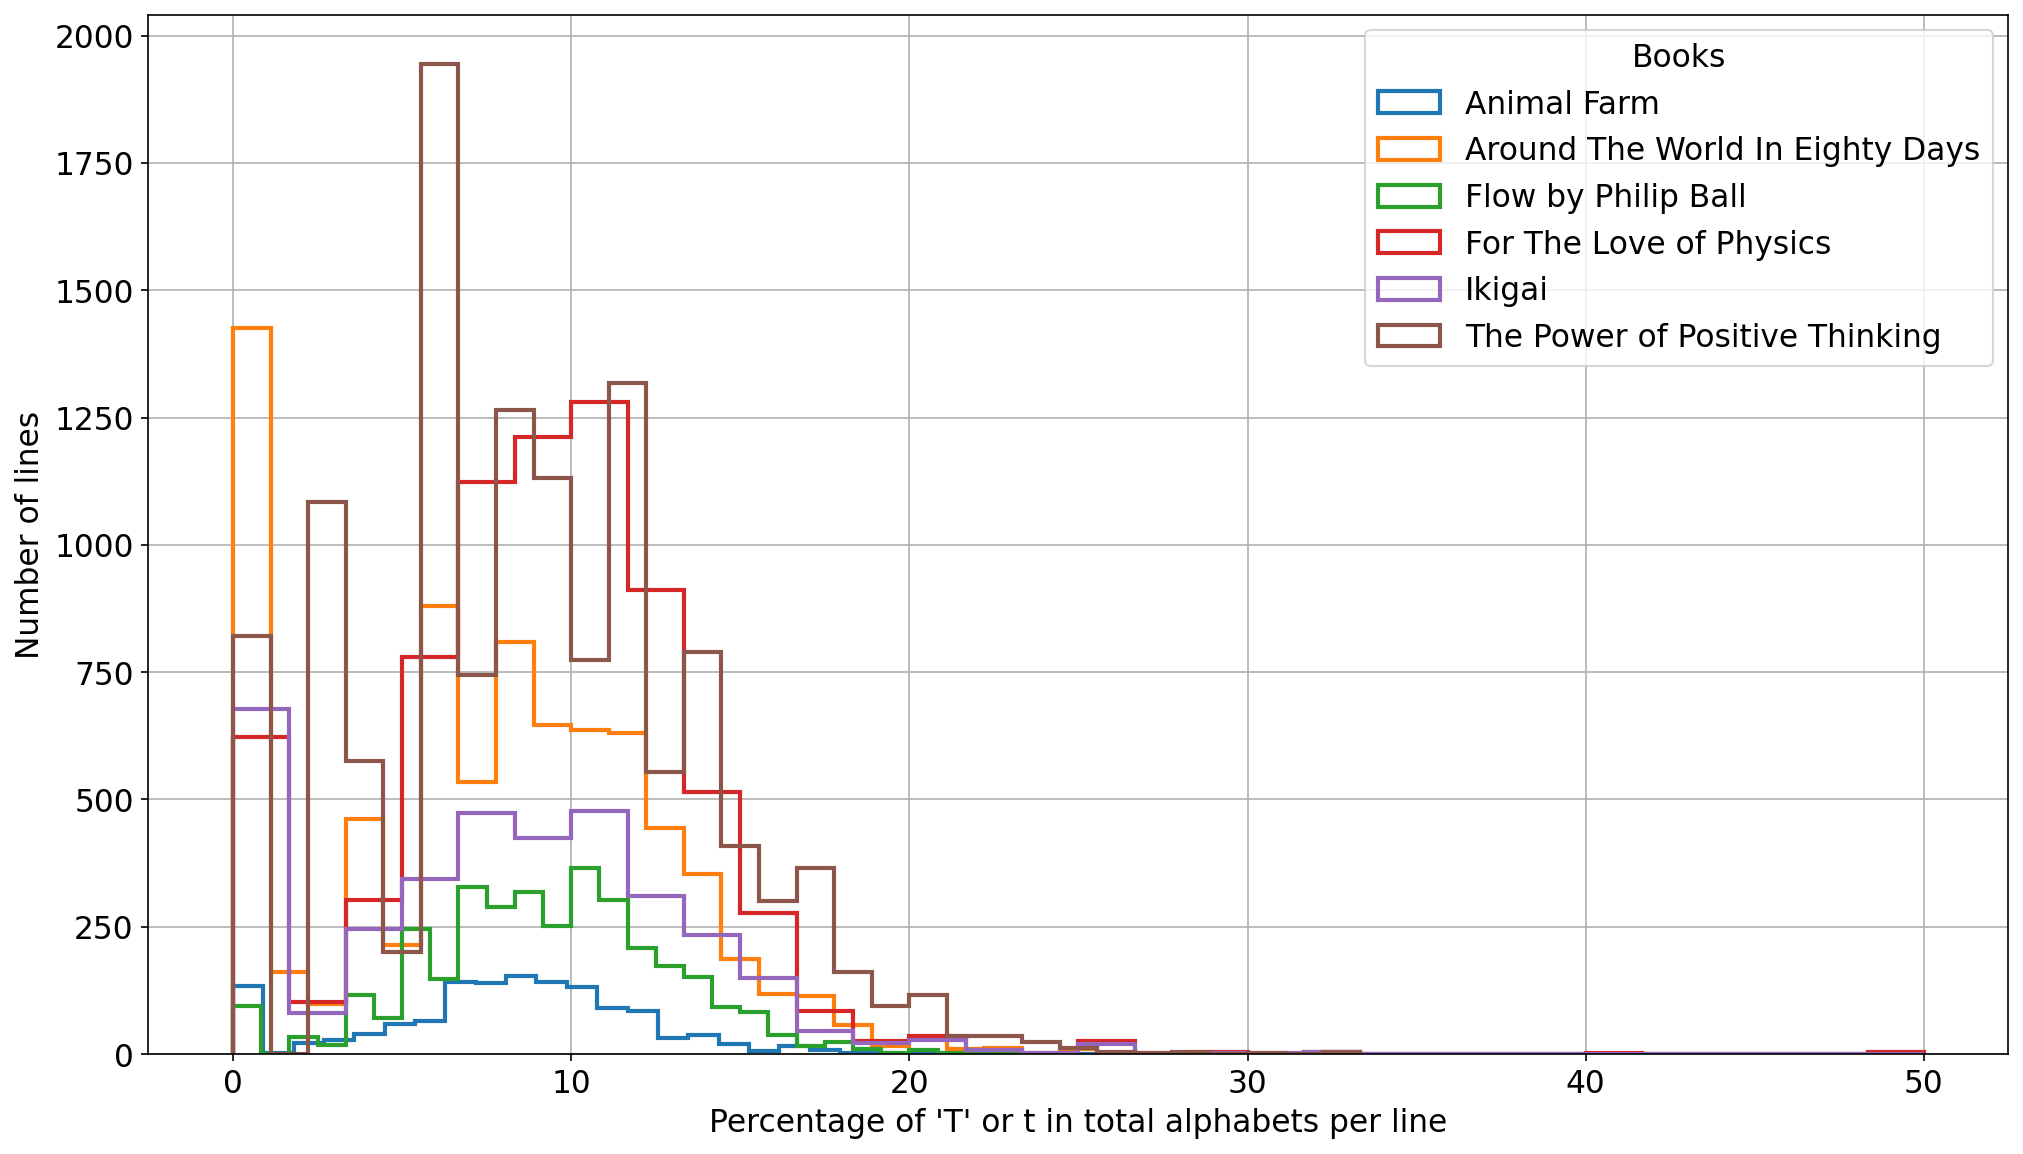
\includegraphics[scale=0.35]{../01_programFiles/histograms/t.png}\hspace{10ex}
    \end{center}
\end{frame}

\begin{frame}
    \frametitle{U or u}
    \begin{center}
        \hspace*{-5ex}
        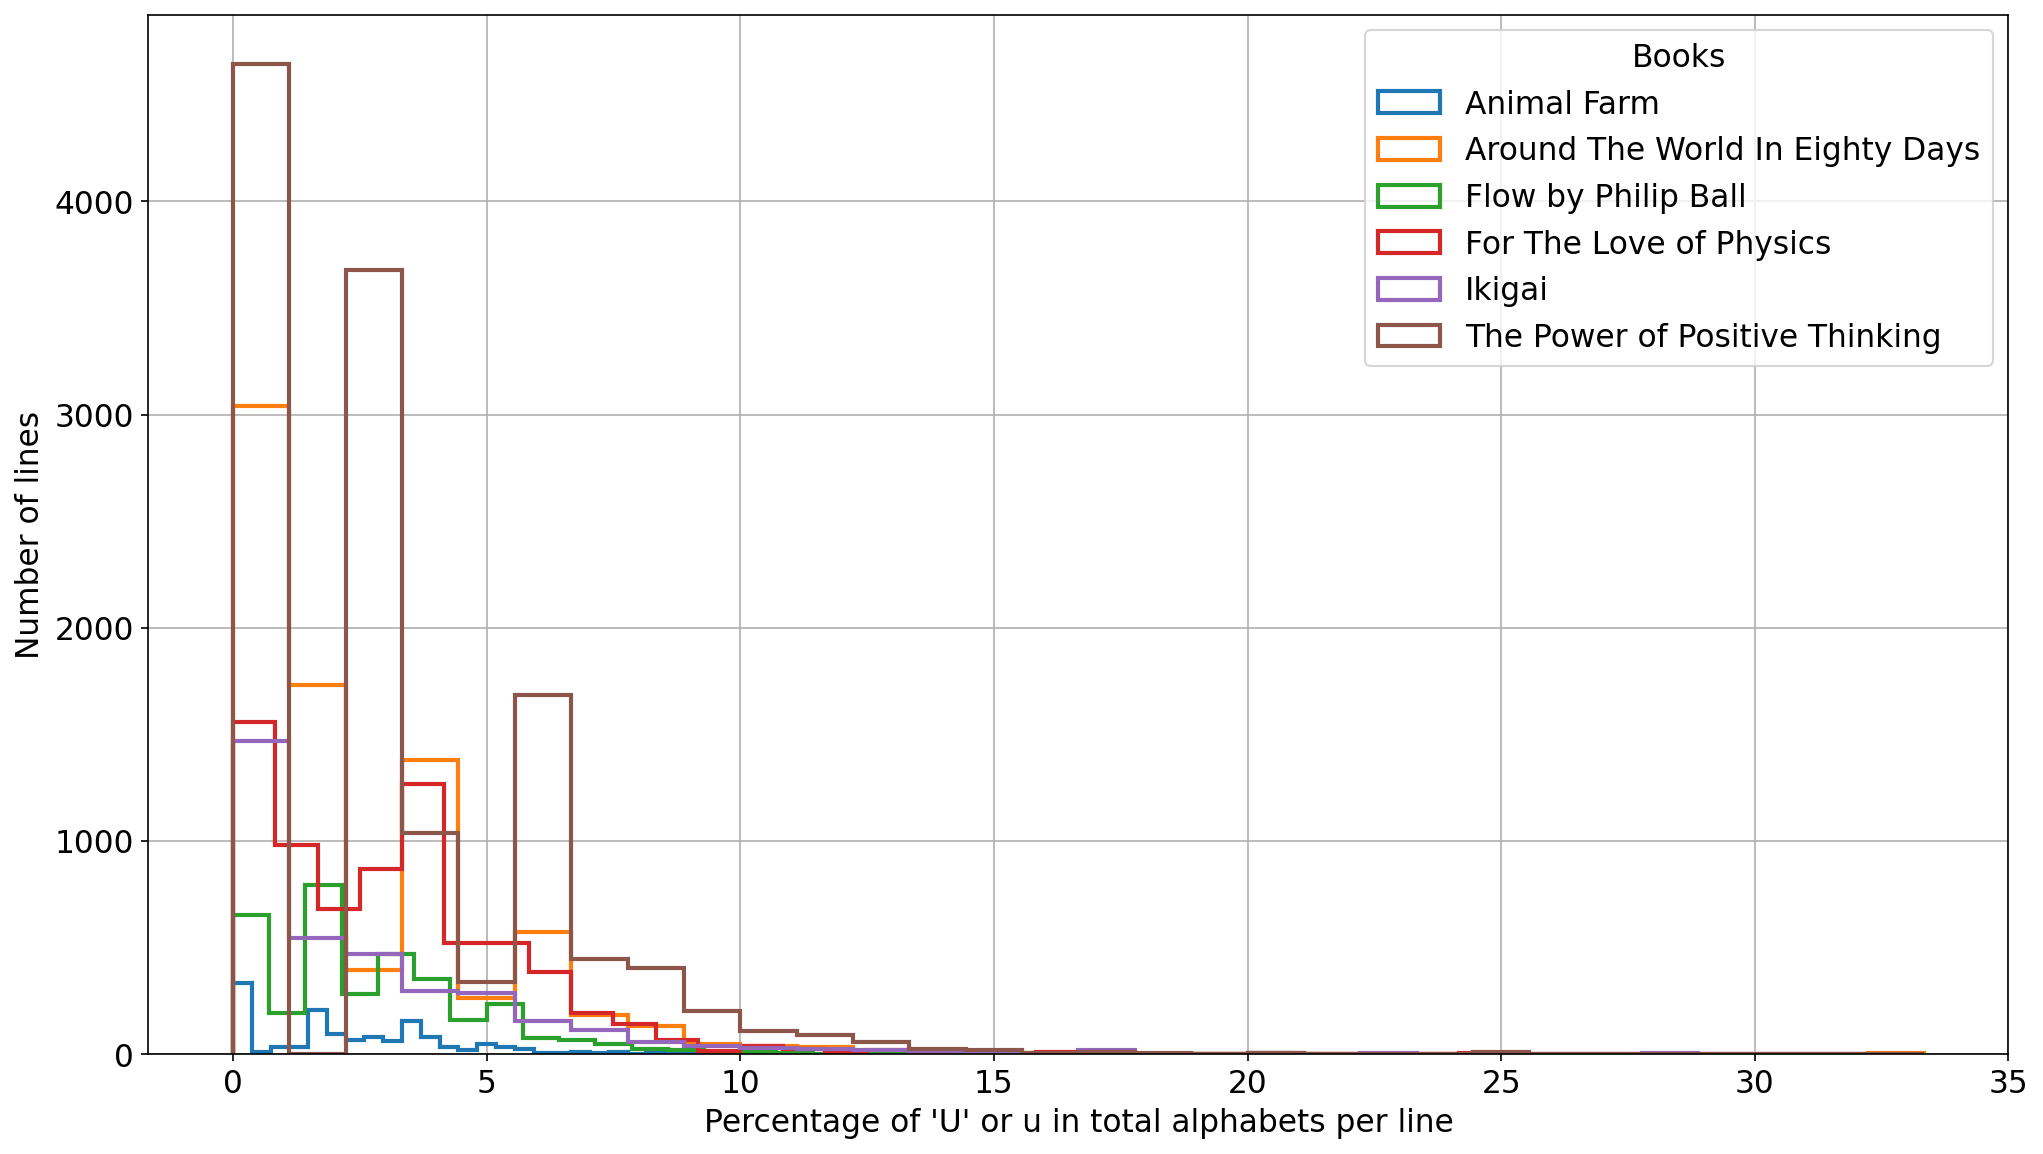
\includegraphics[scale=0.35]{../01_programFiles/histograms/u.png}\hspace{10ex}
    \end{center}
\end{frame}

\begin{frame}
    \frametitle{V or v}
    \begin{center}
        \hspace*{-5ex}
        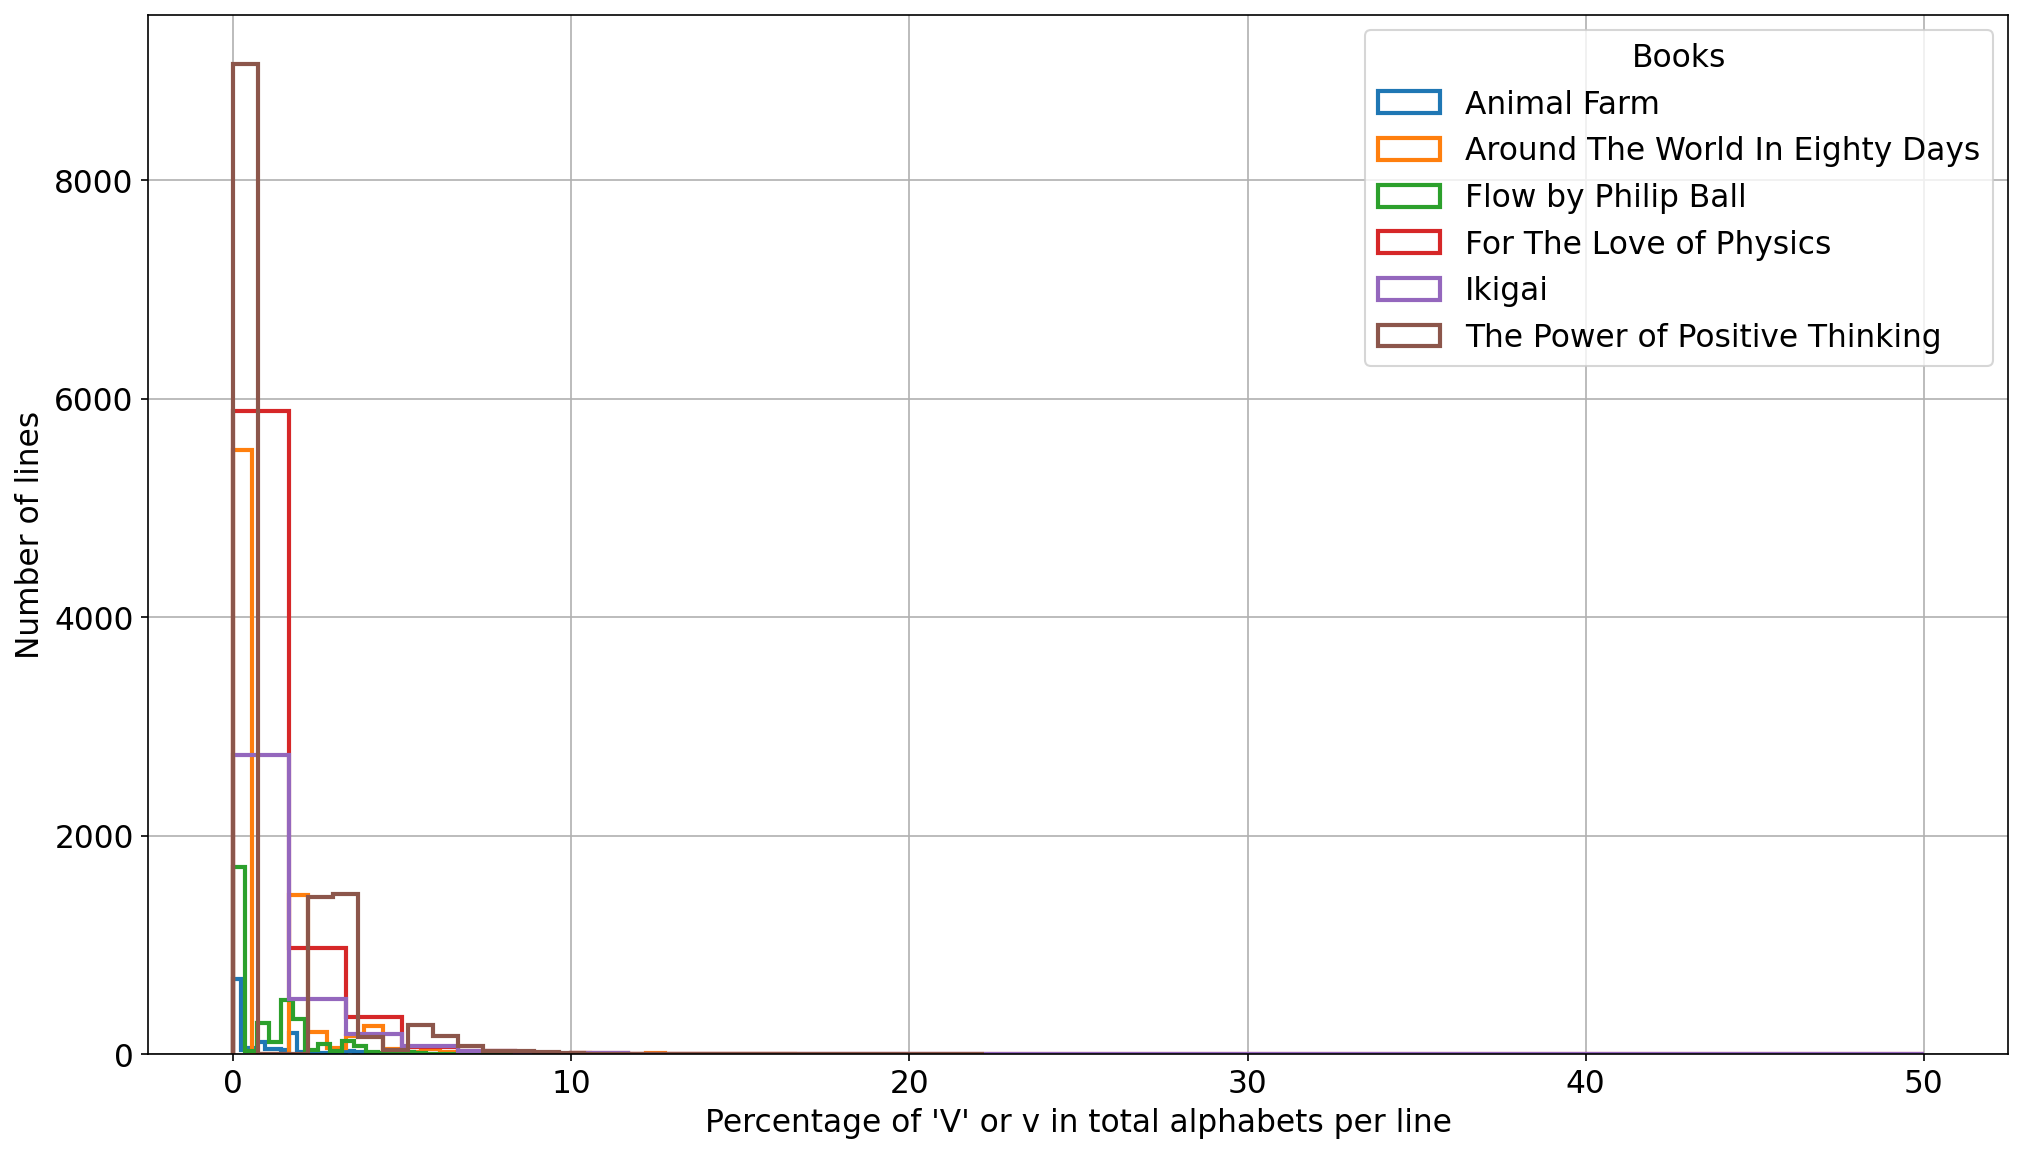
\includegraphics[scale=0.35]{../01_programFiles/histograms/v.png}\hspace{10ex}
    \end{center}
\end{frame}

\begin{frame}
    \frametitle{W or w}
    \begin{center}
        \hspace*{-5ex}
        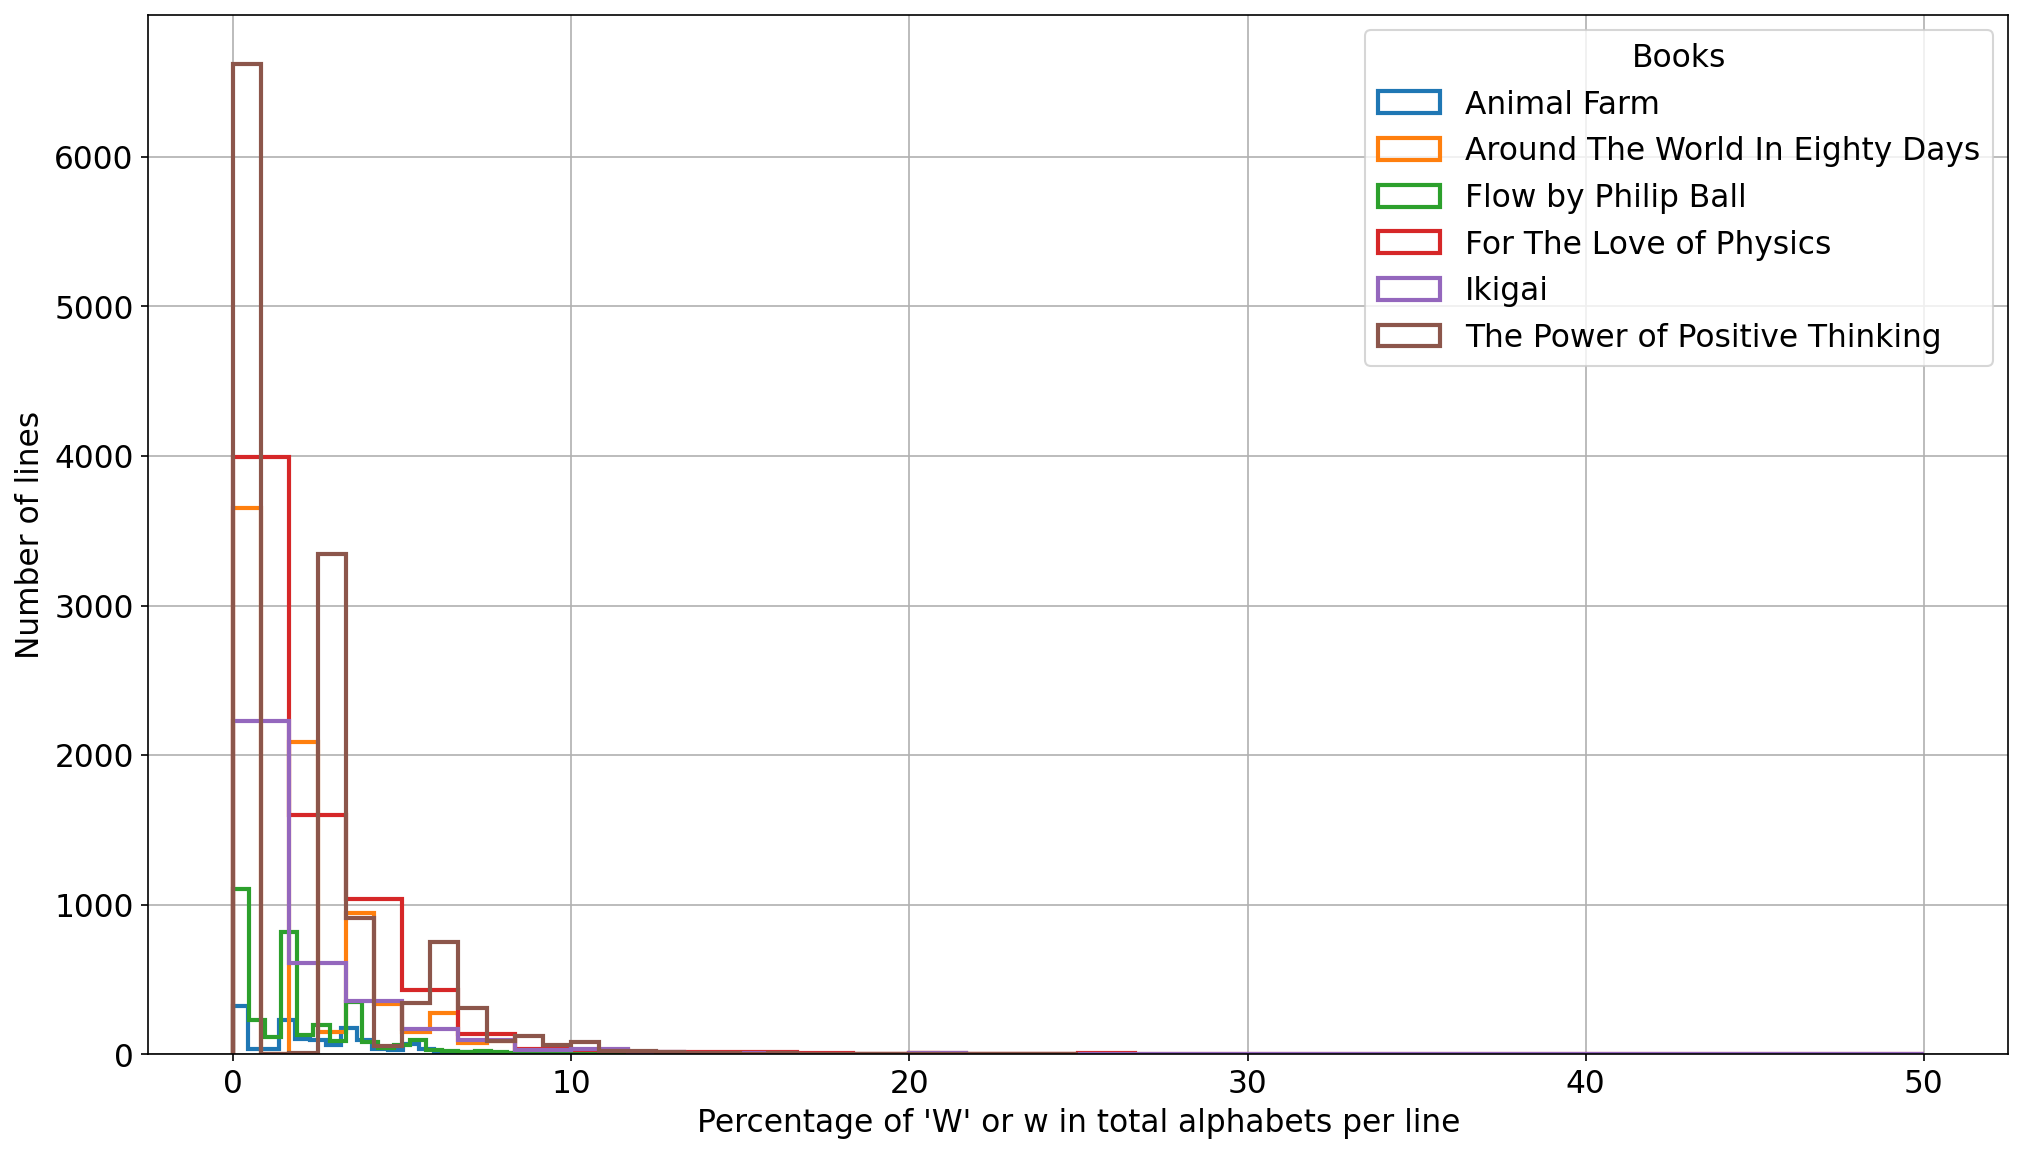
\includegraphics[scale=0.35]{../01_programFiles/histograms/w.png}\hspace{10ex}
    \end{center}
\end{frame}

\begin{frame}
    \frametitle{X or x}
    \begin{center}
        \hspace*{-5ex}
        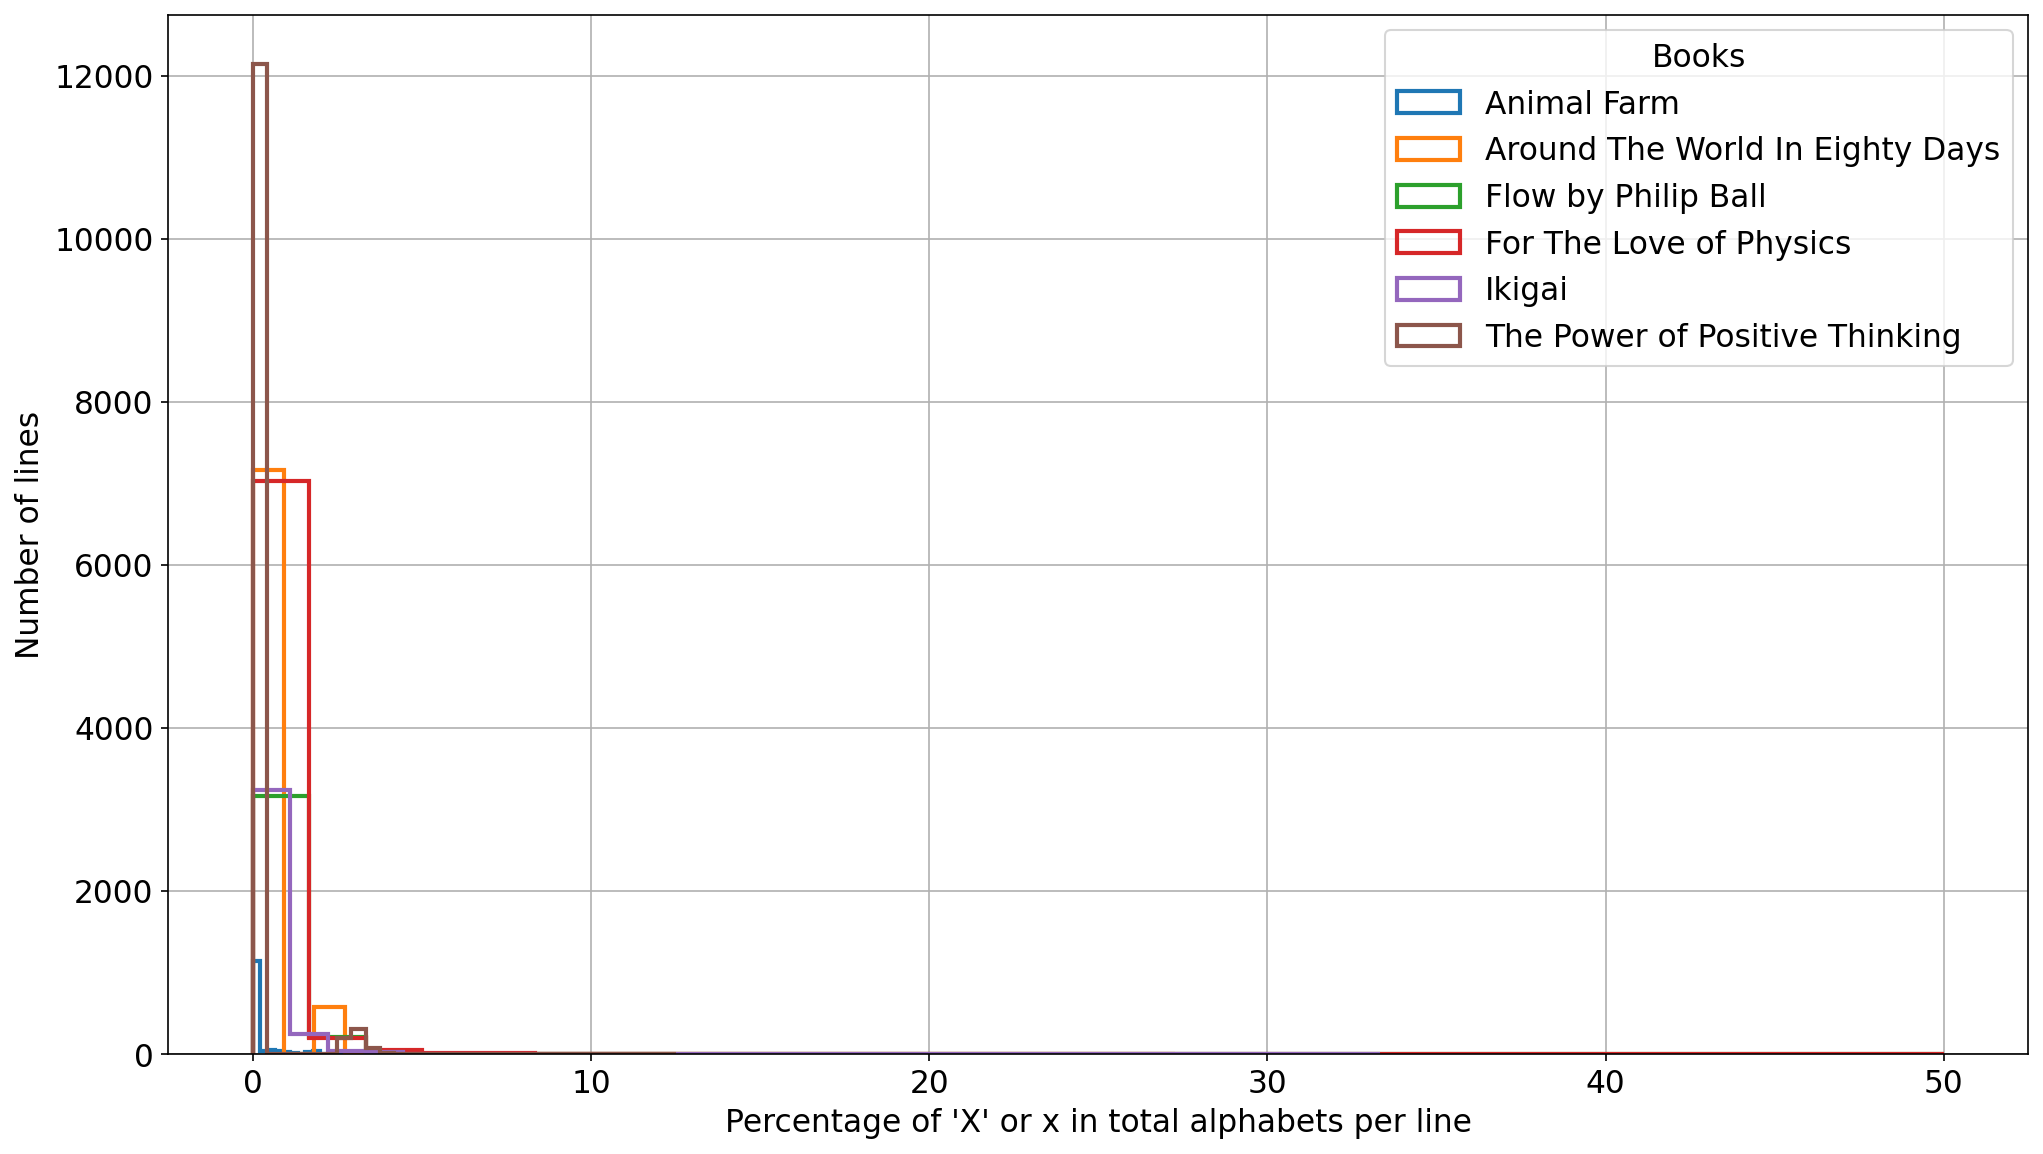
\includegraphics[scale=0.35]{../01_programFiles/histograms/x.png}\hspace{10ex}
    \end{center}
\end{frame}

\begin{frame}
    \frametitle{Y or y}
    \begin{center}
        \hspace*{-5ex}
        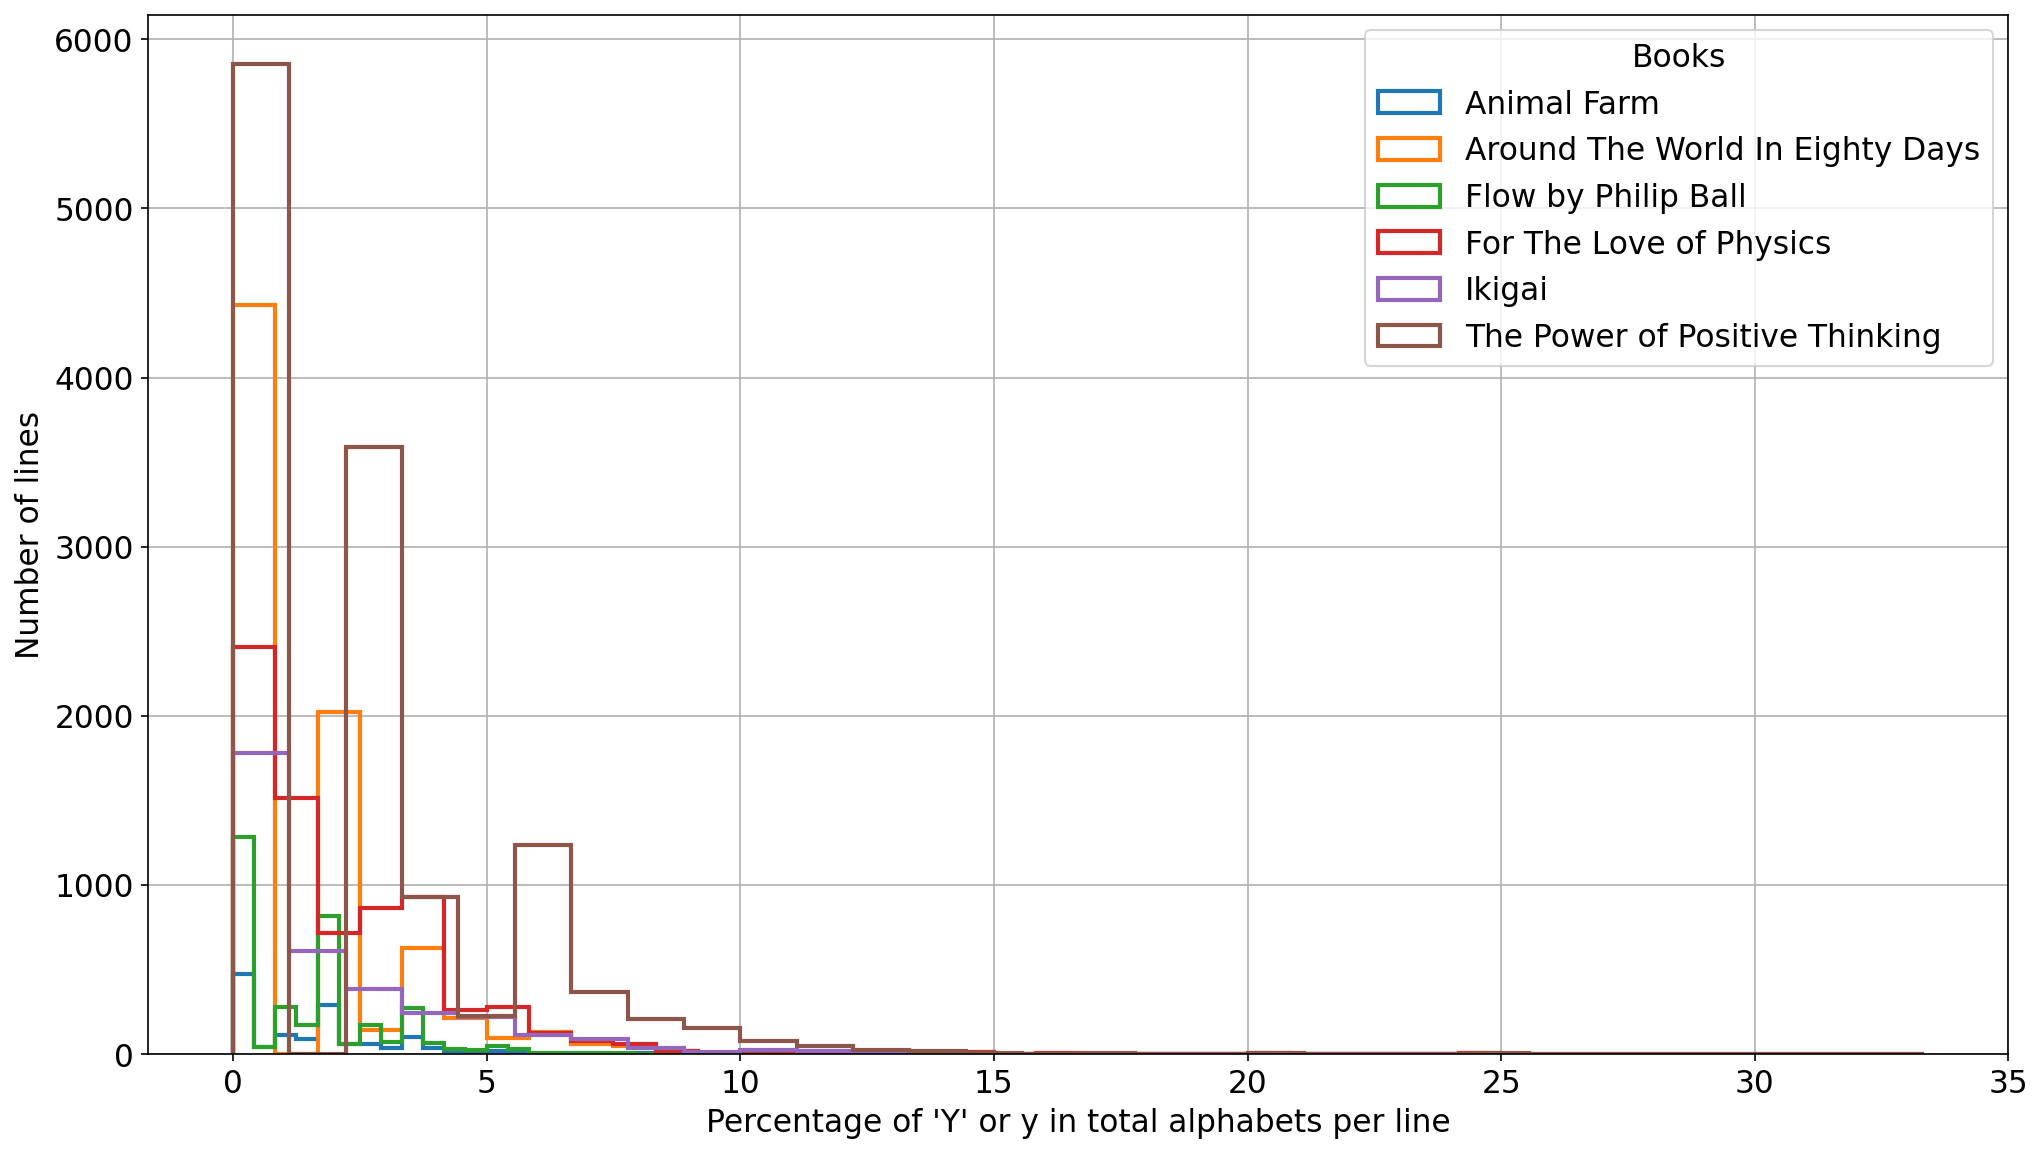
\includegraphics[scale=0.35]{../01_programFiles/histograms/y.png}\hspace{10ex}
    \end{center}
\end{frame}

\begin{frame}
    \frametitle{Z or z}
    \begin{center}
        \hspace*{-5ex}
        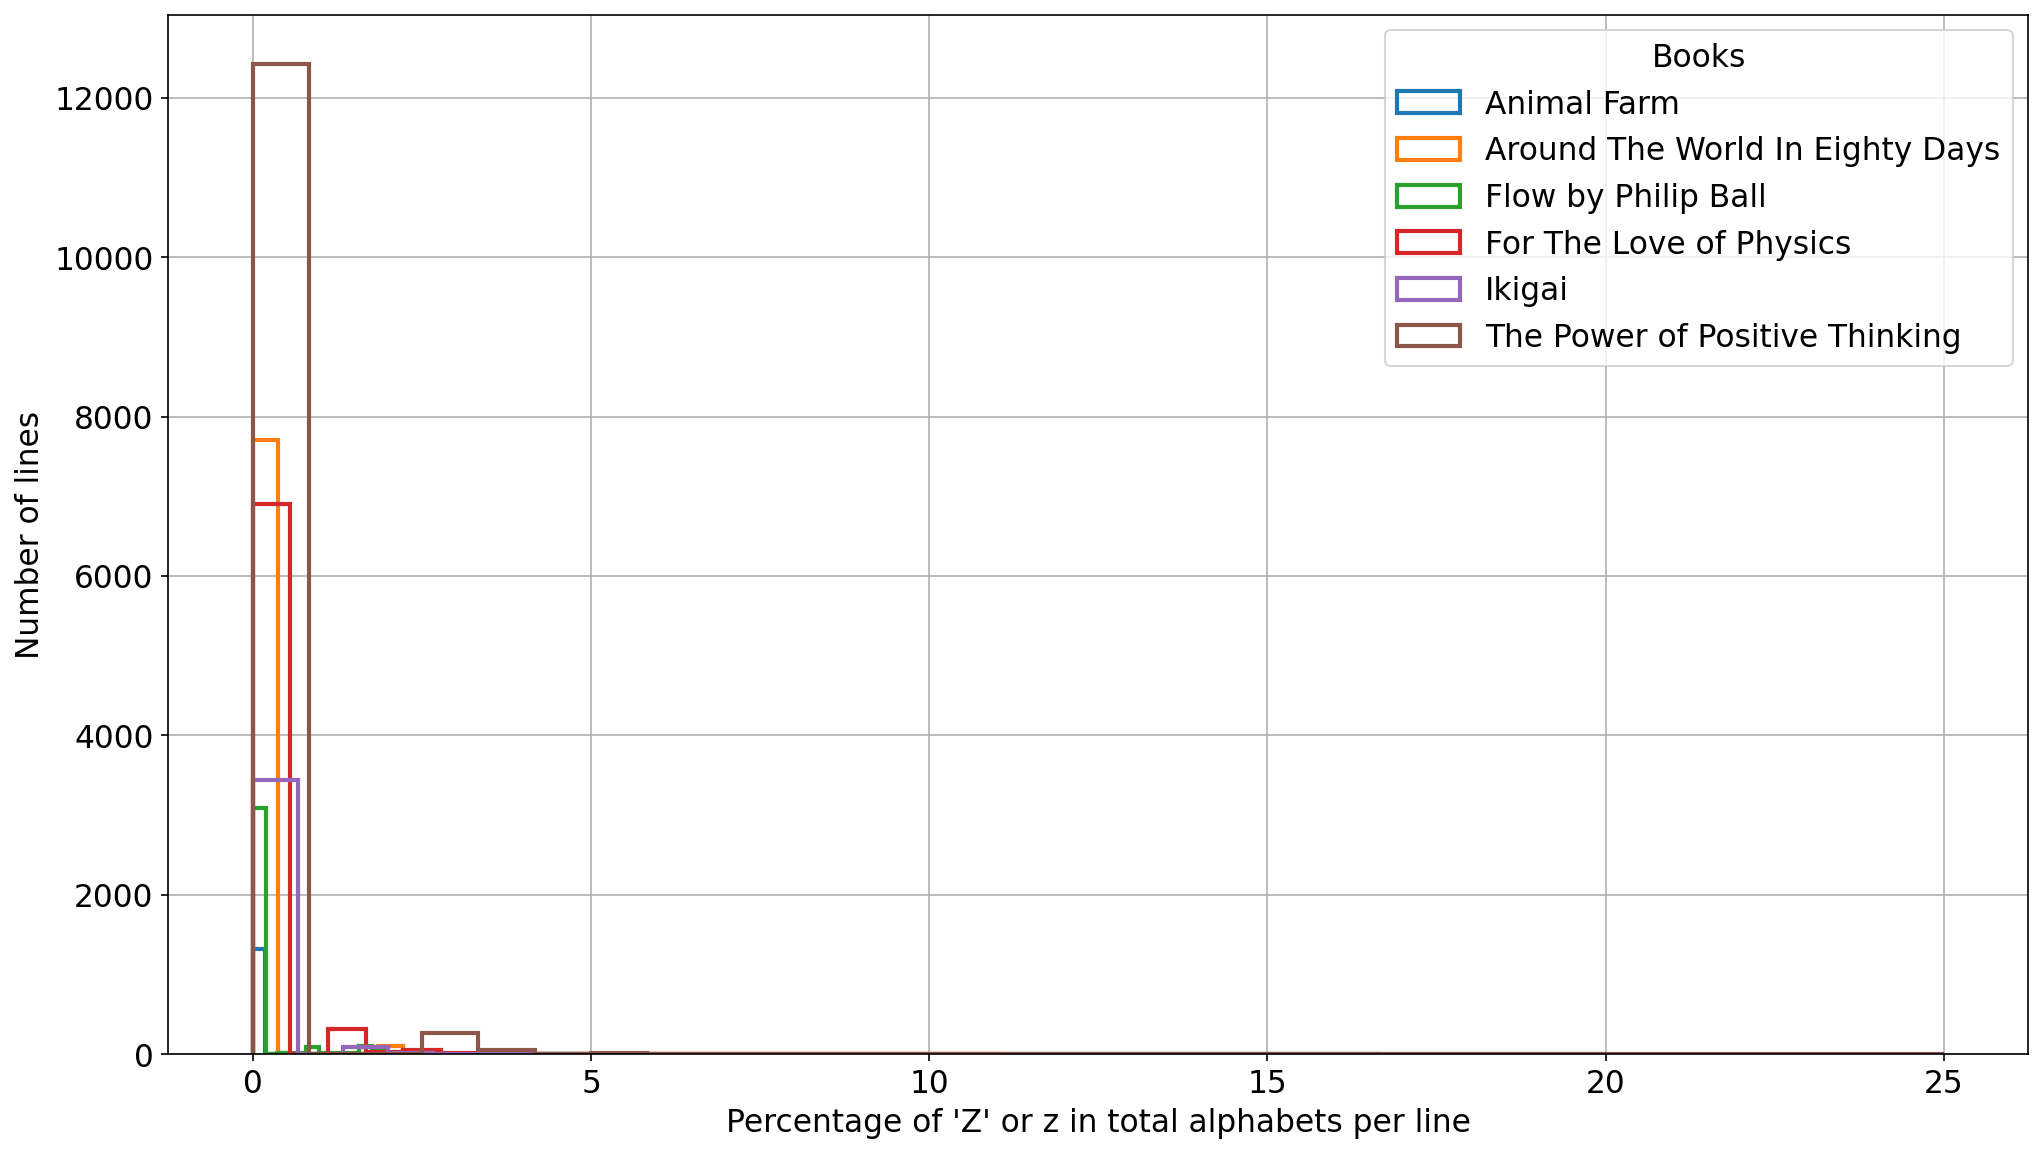
\includegraphics[scale=0.35]{../01_programFiles/histograms/z.png}\hspace{10ex}
    \end{center}
\end{frame}

%------------------------------------------------------------------------------
\begin{frame}
    \frametitle{Observations}

    \begin{itemize}
        \item Least used letters in the chosen books are X, followed by Q and then Z
            \vspace{1cm}
        \item Most used letters in the chosen books are E, followed by A, then O and then T
            \vspace{1cm}
        \item Most used letters appear to follow \textbf{Normal distribution}
            \vspace{1cm}
        \item Least used letters appear to follow \textbf{Exponential distribution}
    \end{itemize}
\end{frame}

%------------------------------------------------------------------------------
\begin{frame}
    \centering
    \usebeamercolor[fg]{title}\usebeamerfont{title} Python code - Reader script
\end{frame}

\begin{frame}[fragile,allowframebreaks]
    \frametitle{Reader script}
    \lstinputlisting[language=python]{../01_programFiles/script_reader.py}
\end{frame}

\begin{frame}
    \centering
    \usebeamercolor[fg]{title}\usebeamerfont{title} Python code - Post-processing script
\end{frame}

\begin{frame}[fragile,allowframebreaks]
    \frametitle{Post-processing script}
    \lstinputlisting[language=python]{../01_programFiles/postProcessing.py}
\end{frame}

\begin{frame}
    \centering
    \usebeamercolor[fg]{title}\usebeamerfont{title} End
\end{frame}

